\documentclass[11pt,a4paper]{article}
\usepackage[margin=2.0cm]{geometry}
\usepackage[T1]{fontenc}
\usepackage[utf8]{inputenc}
\usepackage{lmodern}
\usepackage{microtype}
\usepackage{amsmath,amssymb}
\usepackage{booktabs,array,tabularx}
\usepackage{graphicx}
\usepackage{caption}
\usepackage{placeins}
\usepackage{url}
\usepackage[hidelinks]{hyperref}
\hypersetup{pdftitle={CE634 Assignment 1: Urban Mobility and Ride-Pooling Analysis in New York City}}
\setlength{\parindent}{1.25em}
\setlength{\parskip}{0.25em}
\setlength{\emergencystretch}{2em}
\captionsetup{font=small,skip=5pt,labelfont=bf}
\newcommand{\usd}{\$}
\newcommand{\NN}{\ensuremath{\mathrm{N/N}}}
\newcommand{\YN}{\ensuremath{\mathrm{Y/N}}}
\newcommand{\YY}{\ensuremath{\mathrm{Y/Y}}}
\newcommand{\NY}{\ensuremath{\mathrm{N/Y}}}

\title{\textbf{Urban Mobility, Ride-Pooling Activity, and Within-Cell Comparisons in New York City}\\[0.35em]
\large CE634 Urban Big Data --- Assignment 1}
\author{% TODO: replace before submission
ZHANG Ziqi / 24111604R}
\date{}

\begin{document}
\maketitle

\begin{abstract}
This report analyses New York City Yellow Taxi and High-Volume For-Hire Vehicle (HVFHV) trip records for April and May 2026. The assignment is organized into five tasks covering data auditing, spatial demand and origin--destination (OD) structure, reported ride-pooling activity, travel-time comparison, and passenger-spending comparison. After validity screening, 50,942,185 completed trips are retained. Spatial analysis shows that Yellow Taxi activity is concentrated in Manhattan, whereas HVFHV activity is more geographically distributed and strongly influenced by airport-related demand. The highest-volume OD flows differ markedly from the highest-spending flows, with only two or three pairs overlapping between the respective top-ten rankings. Uber's pooling-request rate is 2.71\% in April and 2.53\% in May, far above Lyft's approximately 0.03\%. Among Uber shared trips with sufficiently populated non-shared reference cells, the median observed travel-time difference is +4.53 min in April and +4.98 min in May. A separate within-cell passenger-spending comparison gives mean shared-minus-reference differences of -\usd8.20 and -\usd8.14. The latter comparisons are descriptive and observational: they quantify differences in recorded trips under explicit matching rules rather than causal effects of ride pooling. The related code and visualizations are available at \url{https://github.com/Arthurqi0825/CE634_Assignment-1}. And visualization results are also available at \url{https://arthurqi0825.github.io/CE634_Assignment-1/}.
\end{abstract}

\section{Introduction}
Large-scale trip records provide a detailed view of how urban mobility is distributed across space, time, service type, and trip purpose. In New York City, the Taxi and Limousine Commission (TLC) publishes monthly Yellow Taxi and High-Volume For-Hire Vehicle (HVFHV) trip records containing pickup and dropoff times, Taxi Zone identifiers, trip characteristics, and monetary fields. HVFHV records additionally report whether a passenger requested a shared ride and whether that request resulted in a reported match with another separately booked passenger \cite{tlc_tripdata,tlc_hvfhv}. These fields support analyses that go beyond total trip counts and allow the assignment to examine spatial demand, ride-pooling activity, travel time, and passenger spending within one consistent data framework.

A key analytical issue is that different indicators answer different questions. A corridor with the largest number of trips is not necessarily the corridor producing the greatest aggregate passenger spending. Likewise, a direct comparison of the raw mean travel time or fare of shared and non-shared trips would mix the effect of trip context with the recorded pooling status because the two groups can differ in OD distribution, pickup time, and other observed characteristics. The analysis therefore combines descriptive spatial statistics with explicit within-cell reference comparisons.

The report retains the assignment's task-by-task organization so that each required output can be verified directly. Task 1 establishes the retained analysis population and the observed request/match states. Task 2 describes pickup/dropoff demand and compares directed OD rankings by trip volume and aggregate passenger spending. Task 3 quantifies platform-specific pooling requests, reported matches, and matching success. Task 4 compares the observed travel time of supported Uber shared trips with non-shared trips in comparable OD--time cells. Task 5 compares observed passenger spending under a related matching design. Across Tasks 4 and 5, reference coverage is reported alongside the effect-size summary because unsupported shared trips are deliberately left unmatched rather than assigned an artificial reference.

\section{Data and Analysis Framework}
\subsection{Data sources and study period}
The analysis uses April and May 2026 TLC Yellow Taxi and HVFHV trip records, together with the official Taxi Zone lookup table and Taxi Zone boundary files. TLC describes the monthly files as provider-submitted operational records and notes that complete accuracy cannot be guaranteed; the results should therefore be interpreted as patterns in recorded service activity rather than a perfect census of all mobility behaviour \cite{tlc_tripdata}. Taxi Zones are approximate neighborhood-scale spatial units and provide the common geography for pickup, dropoff, and OD analysis \cite{tlc_zoneguide}.

The HVFHV license identifier is used to distinguish Juno (HV0002), Uber (HV0003), Via (HV0004), and Lyft (HV0005). In the retained April--May files, only Uber and Lyft contain observations. Yellow Taxi records do not contain the HVFHV request/match variables and therefore contribute to the trip-count, spatial, OD, and spending analyses but not to the ride-pooling-status analysis.

\subsection{General validity rules}
A completed trip requires valid pickup and dropoff timestamps, pickup during the relevant study month, and a dropoff later than the pickup. Additional validity checks are applied only to analyses that require the corresponding variables. Spatial and OD analysis requires valid Taxi Zone identifiers; spending analysis requires valid monetary components; and travel-time analysis requires a positive, plausible recorded duration. This task-specific screening avoids discarding an otherwise usable trip because an unrelated field is invalid.

The TLC HVFHV dictionary defines \texttt{shared\_request\_flag} as whether the passenger agreed to a shared/pooled ride and \texttt{shared\_match\_flag} as whether the passenger was matched with another separately booked passenger during the trip \cite{tlc_hvfhv}. These two fields define four recorded states: \NN{} (no request/no match), \YN{} (request/no match), \YY{} (request/match), and \NY{} (no request/match). The rare \NY{} state is retained as an observed inconsistency rather than silently recoded.

For Yellow Taxi, recorded passenger spending is represented by \texttt{total\_amount}. For HVFHV, spending is constructed from the relevant passenger-paid fare components, including the base passenger fare, tolls, Black Car Fund contribution, sales tax, congestion surcharge, airport fee, tips, and CBD congestion fee; driver pay is excluded. Non-finite components are not replaced with zero, and negative total spending is excluded from spending comparisons as a likely correction or refund.

\section{Task 1: Data Audit and Retained Trip Population}
\subsection{Objective and method}
Task 1 establishes the usable sample before any spatial or pooling analysis is performed. The main outputs are the number of retained completed trips by service and month and, for HVFHV records, the distribution of the four request/match states. Separating this audit from later analyses makes the denominators transparent and identifies which platforms provide sufficient shared-trip observations for Tasks 3--5.

\subsection{Results and interpretation}
The audit starts from 51,043,773 raw records and retains 50,942,185 completed trips for the principal count analysis. The cleaning rules are applied only when the corresponding field is required. Thus, nonpositive duration excludes a trip from completed-trip counts, OD analysis, and later duration analysis, whereas negative passenger spending affects spending summaries but not demand counts. Table~\ref{tab:audit} gives the main diagnostic counts and selected overlap information used to check whether exclusions are additive. The two largest overlaps are request-after-pickup with invalid on-scene order (544,494 records) and negative payment with negative base fare (33,131 records), so the audit flags should not be summed as independent exclusions.

\begin{table}[!htbp]
\centering
\caption{Selected data-quality flags and retained records by analysis.}
\label{tab:audit}
\small
\begin{tabular}{lrr}
\toprule
Audit item & April 2026 & May 2026 \\
\midrule
Raw pickup records: Yellow Taxi & 3,831,239 & 4,090,823 \\
Raw pickup records: HVFHV & 20,995,953 & 22,125,744 \\
Nonpositive duration records & 49,511 & 52,063 \\
Nonpositive distance records & 95,372 & 115,316 \\
Negative passenger-spending records & 17,109 & 17,236 \\
HVFHV request after pickup & 268,958 & 275,536 \\
HVFHV invalid request/on-scene/pickup order & 362,125 & 402,971 \\
HVFHV N/Y sharing-flag inconsistency & 783 & 1,177 \\
\midrule
Retained completed trips & 24,777,681 & 26,164,504 \\
Retained spending records & 24,760,572 & 26,147,268 \\
Retained distance-dependent records & 24,681,469 & 26,047,976 \\
Retained HVFHV sharing-status records & 20,995,953 & 22,125,744 \\
\bottomrule
\end{tabular}
\end{table}

Across April and May, Uber accounts for 60.33\% of the retained completed-trip sample, Lyft for 24.32\%, and Yellow Taxi for 15.35\%. Table~\ref{tab:sample} reports the requested Task 1.2 categories, using the request flag first and the match flag second. Juno (HV0002), Via (HV0004), and other HVFHV company codes have no retained observations in the April--May files, so the Uber and Lyft subtotals reconcile exactly to the HVFHV total. Yellow Taxi has no specified sharing status and is therefore reported only as all retained trips.

\begin{table}[!htbp]
\centering
\caption{Retained trips by service and request/match category.}
\label{tab:sample}
\small
\begin{tabularx}{\linewidth}{>{\raggedright\arraybackslash}p{3.0cm}>{\raggedright\arraybackslash}Xrr}
\toprule
Service & Request/match category & April trips & May trips \\
\midrule
Yellow Taxi & All retained trips & 3,781,728 & 4,038,760 \\
HVFHV & All retained trips & 20,995,953 & 22,125,744 \\
\midrule
Uber & \NN{} & 14,961,455 & 14,966,066 \\
Uber & \YN{} & 162,018 & 167,846 \\
Uber & \YY{} & 255,385 & 220,904 \\
Uber & \NY{} & 0 & 0 \\
Uber & Missing or other statuses & 0 & 0 \\
\midrule
Lyft & \NN{} & 5,614,374 & 6,767,729 \\
Lyft & \YN{} & 1,865 & 1,954 \\
Lyft & \YY{} & 73 & 68 \\
Lyft & \NY{} & 783 & 1,177 \\
Lyft & Missing or other statuses & 0 & 0 \\
\midrule
Juno, Via, and other HVFHV codes & All retained trips & 0 & 0 \\
\midrule
Total & All retained completed trips & 24,777,681 & 26,164,504 \\
\bottomrule
\end{tabularx}
\end{table}

Figure~\ref{fig:dataset} combines the service-level sample size with the observed HVFHV request/match composition. The key point is that reported matched shared trips are a small subset of the full HVFHV population and are overwhelmingly supplied by Uber. Lyft contributes only 141 \YY{} trips across the two months and also contains all observed \NY{} records. This sample structure motivates the later decision to focus the travel-time comparison on Uber rather than treating Uber and Lyft as equally supported platforms.

\begin{figure}[!htbp]
\centering
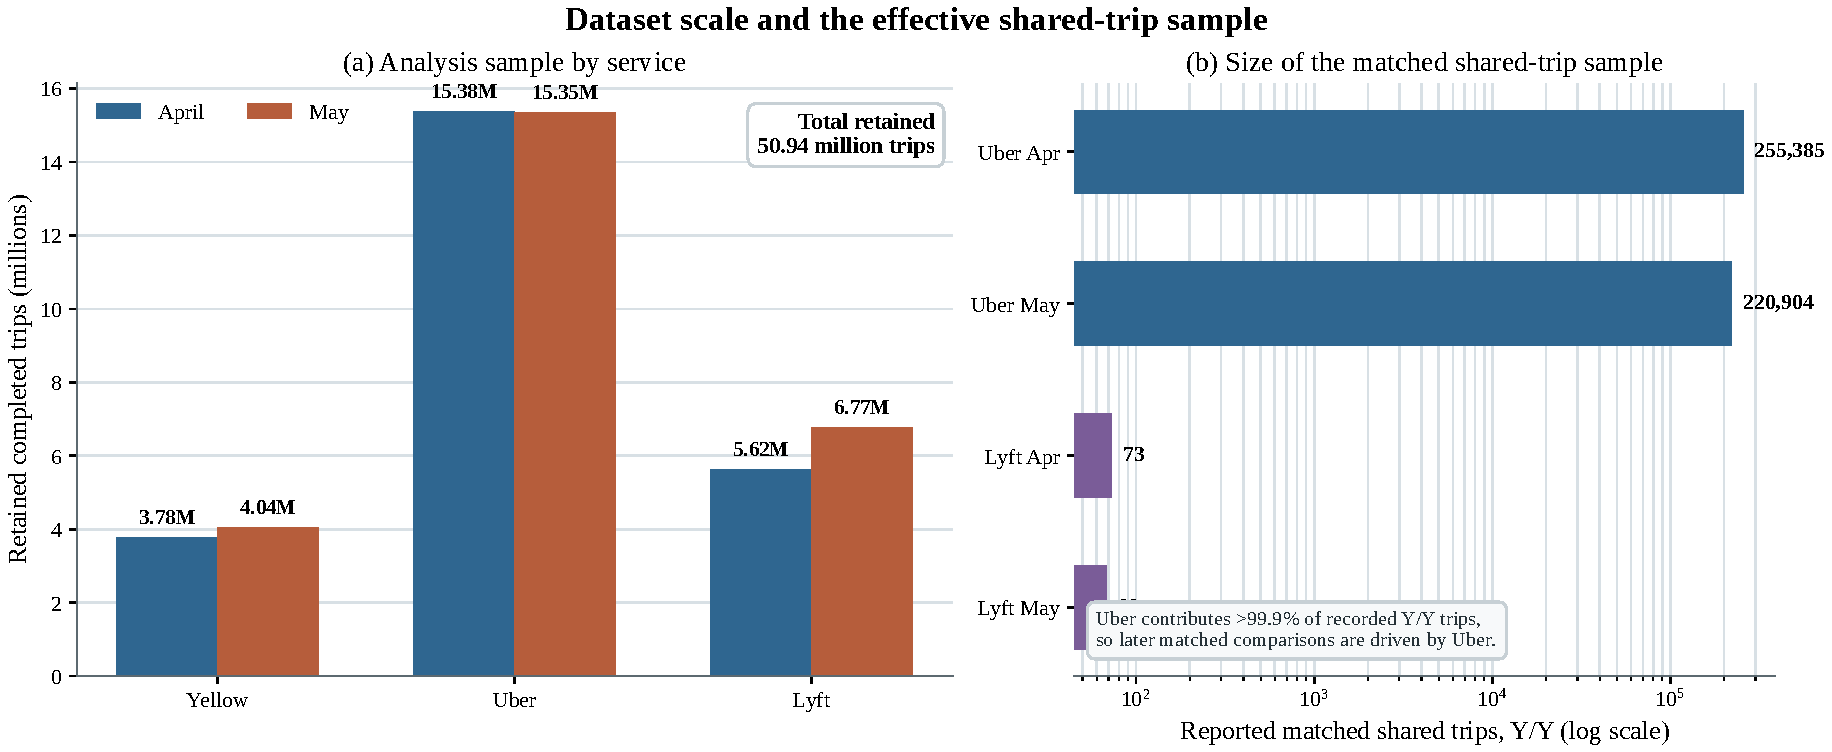
\includegraphics[width=.98\linewidth]{04_Results/paper_figures/main/fig1_dataset_overview.pdf}
\caption{\textbf{Dataset overview and reported shared-trip support.} The left panel summarizes retained completed trips by service and month. The right-side annotations highlight the size of the reported \YY{} sample available for later comparisons. Uber contributes essentially all recorded matched shared trips, whereas Lyft contributes only a very small sample.}
\label{fig:dataset}
\end{figure}
\FloatBarrier

\section{Task 2: Spatial Demand and Directed OD Analysis}
\subsection{Method}
Pickup and dropoff demand are calculated as counts of completed trips by TLC Taxi Zone. Logarithmic color scales are used because zone counts span several orders of magnitude. Zone 265 (Outside of NYC) is a valid TLC lookup category but has no drawable polygon; it is retained in all tables and OD rankings even though it cannot be colored on the choropleth maps.

Directed OD analysis treats $A\rightarrow B$ and $B\rightarrow A$ as different flows and retains within-zone trips $A\rightarrow A$. For each month and service, OD pairs are ranked independently by (i) completed-trip count and (ii) aggregate recorded passenger spending. Comparing the two top-ten rankings tests whether the corridors with the most trips are also the corridors with the greatest monetary magnitude.

\subsection{Pickup and dropoff demand}
Figures~\ref{fig:spatial_apr} and \ref{fig:spatial_may} place the eight required Task 2.1 hotspot maps in the main report rather than in the appendix: for each month, the four panels show Yellow Taxi pickups, Yellow Taxi dropoffs, HVFHV pickups, and HVFHV dropoffs. They show a stable contrast between Yellow Taxi and HVFHV activity. Yellow Taxi pickup and dropoff demand is concentrated in Manhattan. In April, the highest Yellow pickup counts occur in Upper East Side South (179,336), Midtown Center (161,098), and Upper East Side North (158,209). In May, the corresponding leading zones are Upper East Side South (194,209), Upper East Side North (172,093), and Midtown Center (158,714). The geographic concentration is therefore persistent across both months.

HVFHV demand is more dispersed. The leading drawable pickup zones are LaGuardia Airport, JFK Airport, and Crown Heights North in both months. LaGuardia increases from 412,983 pickups in April to 453,507 in May, while JFK increases from 318,541 to 365,545. HVFHV dropoffs to the non-drawable Outside of NYC category are even larger: 930,707 in April and 1,018,509 in May. Reporting this category explicitly prevents the map geometry from hiding an important destination pattern.

\begin{figure}[!htbp]
\centering
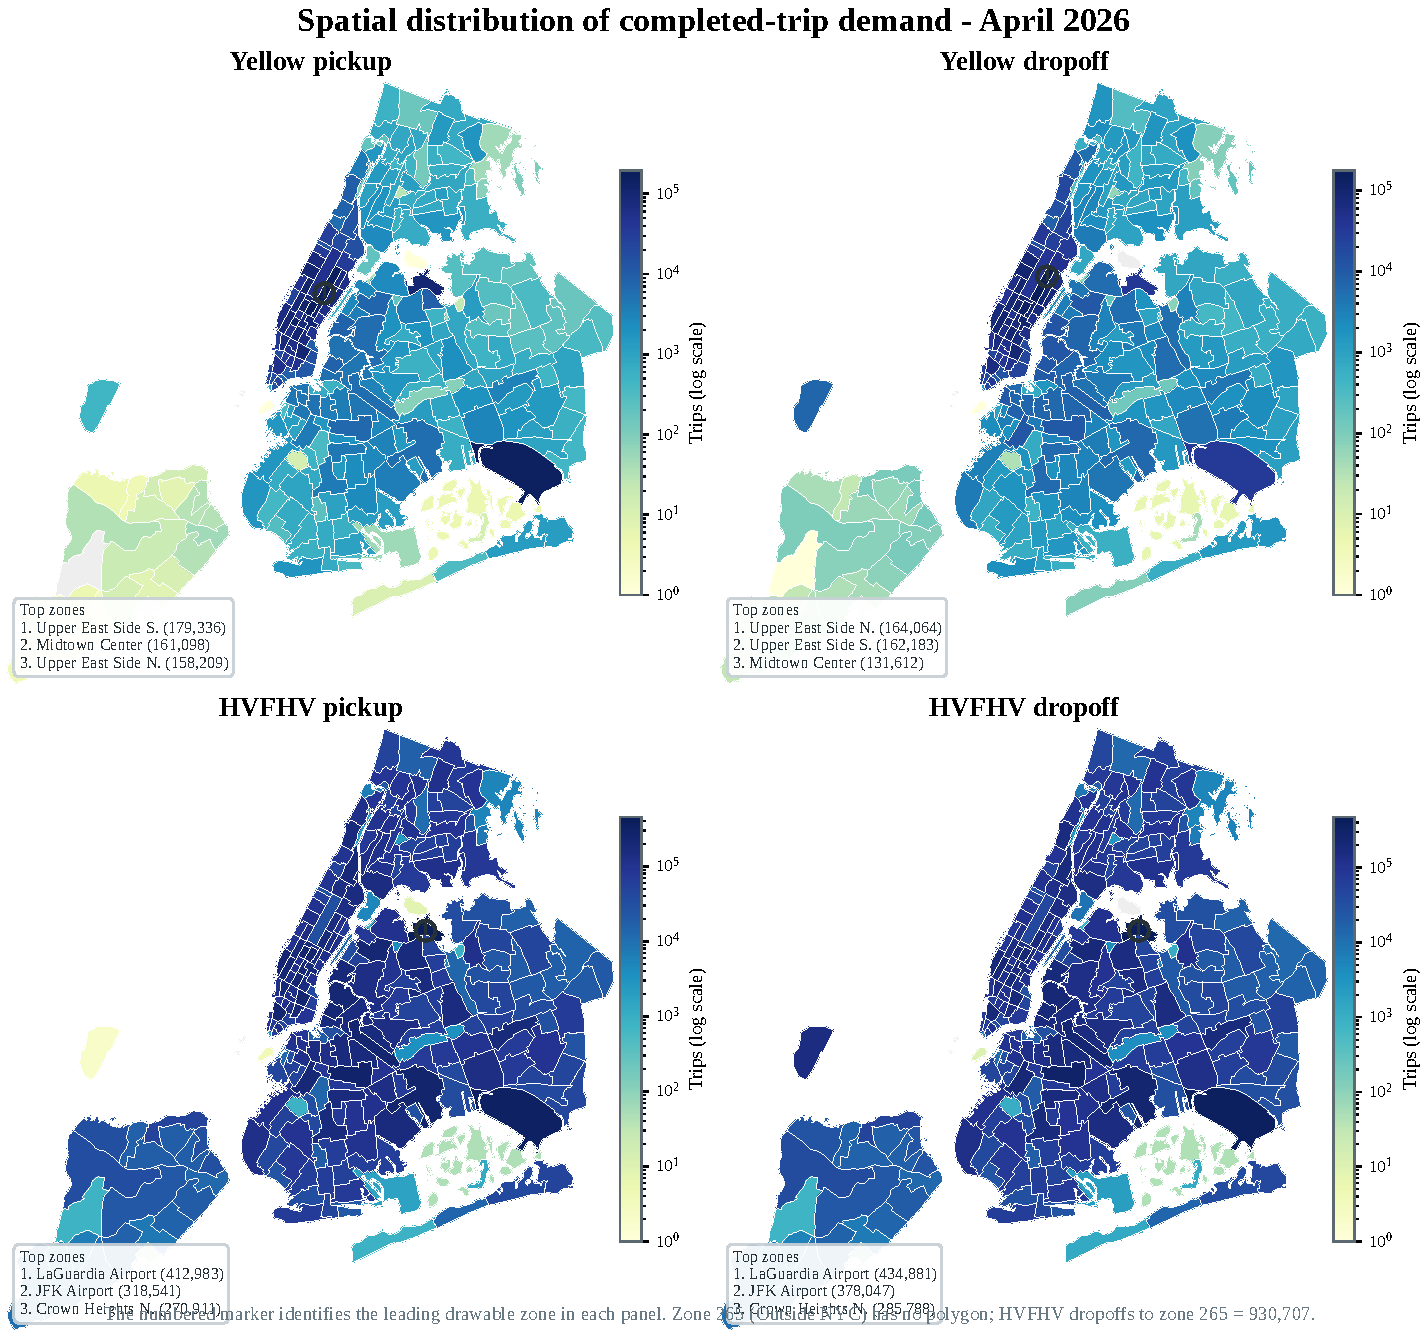
\includegraphics[width=.91\linewidth]{04_Results/paper_figures/main/fig2_spatial_demand_april.pdf}
\caption{\textbf{Task 2.1 hotspot maps for April 2026.} The four main-text panels show Yellow Taxi origins, Yellow Taxi destinations, HVFHV origins, and HVFHV destinations. Each panel lists its three leading drawable zones and marks the highest-count drawable zone directly on the map. Yellow Taxi demand is strongly Manhattan-centered, whereas HVFHV demand is more geographically distributed and shows strong airport activity. Zone 265 is counted in the analysis but cannot be colored because no polygon is provided.}
\label{fig:spatial_apr}
\end{figure}

\begin{figure}[!htbp]
\centering
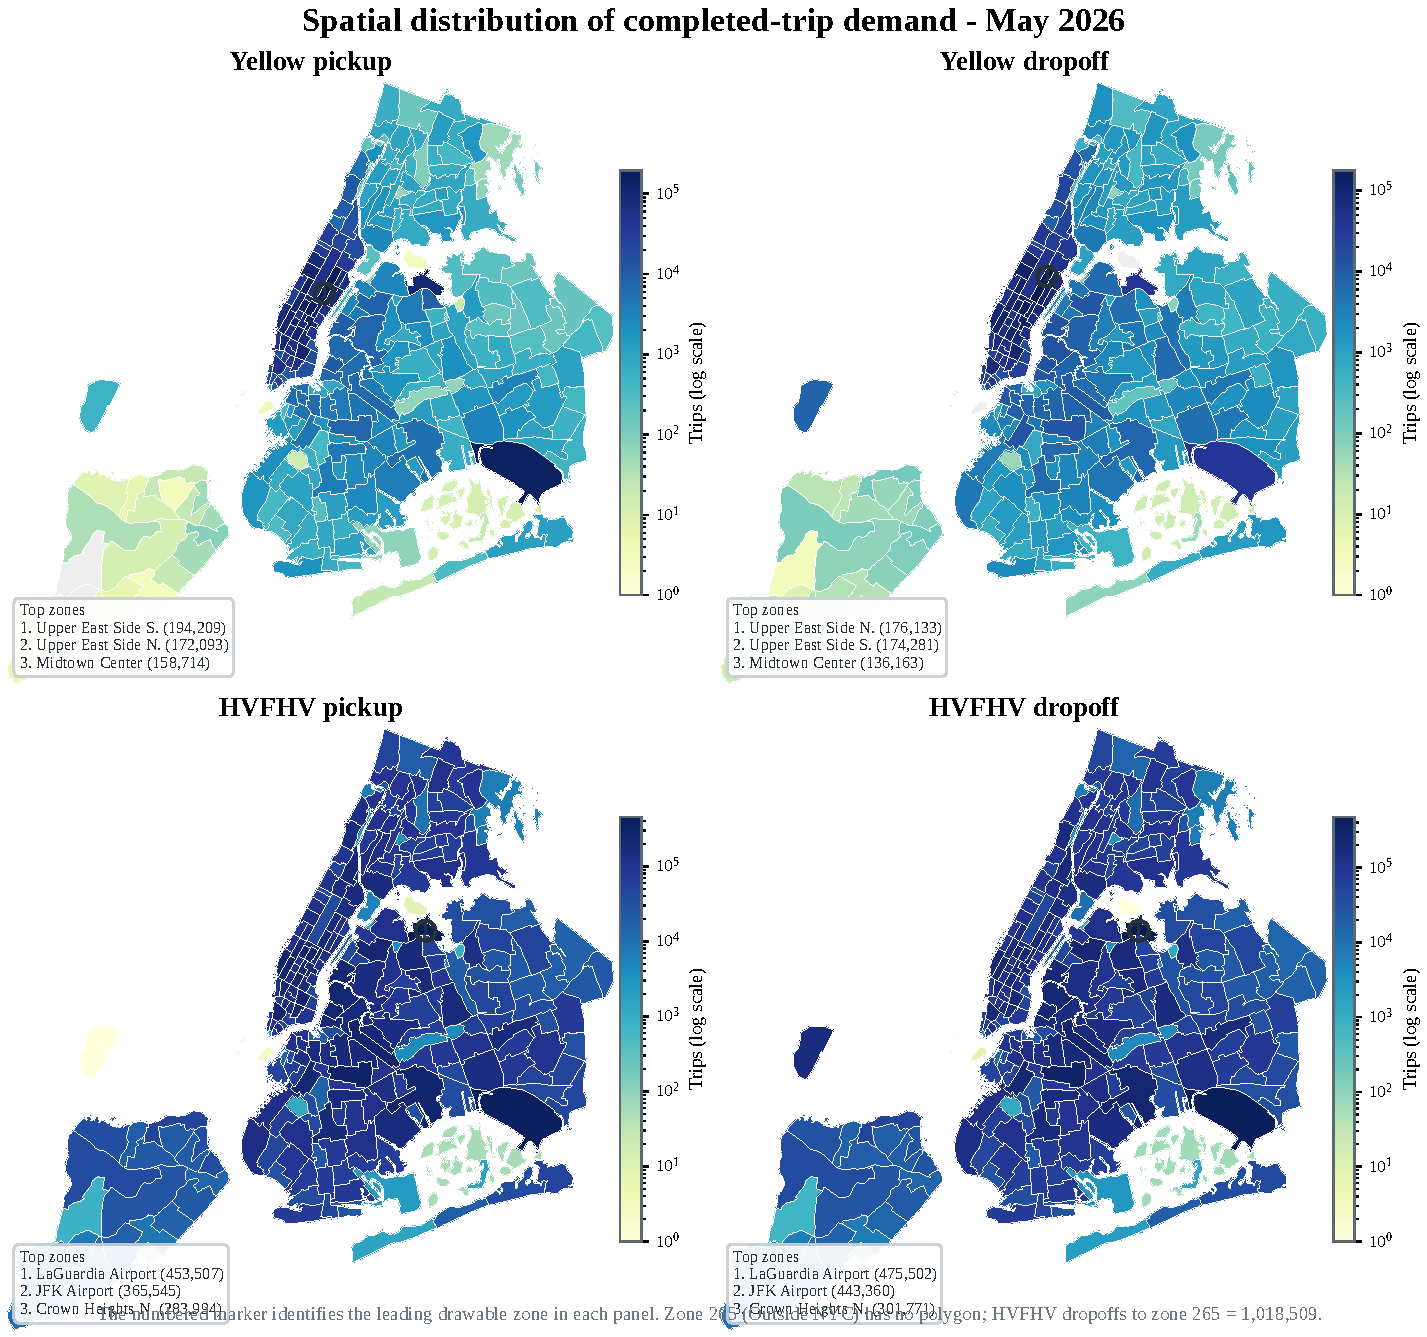
\includegraphics[width=.91\linewidth]{04_Results/paper_figures/main/fig3_spatial_demand_may.pdf}
\caption{\textbf{Task 2.1 hotspot maps for May 2026.} The four main-text panels show Yellow Taxi origins, Yellow Taxi destinations, HVFHV origins, and HVFHV destinations. The same service/measure scales are used as in April to support month-to-month comparison. The main spatial pattern remains stable, while several airport and Manhattan zones record higher counts.}
\label{fig:spatial_may}
\end{figure}

\subsection{Volume versus passenger spending}
The OD rankings show that trip frequency and aggregate passenger spending identify different mobility structures. In both months, the highest-volume Yellow Taxi OD pair is Upper East Side South (237) $\rightarrow$ Upper East Side North (236). For Uber and Lyft, the highest-volume pair is East New York (76) $\rightarrow$ East New York (76), a high-frequency within-zone movement.

The spending rankings point elsewhere. For Yellow Taxi and Uber, JFK Airport (132) $\rightarrow$ Outside of NYC (265) is the leading OD pair by aggregate spending in both months. Lyft is led by LaGuardia Airport (138) $\rightarrow$ Outside of NYC in April and JFK Airport $\rightarrow$ Outside of NYC in May. Only 3 of Yellow's 10 highest-volume OD pairs also appear in its spending top ten, and only 2 of 10 overlap for Uber and Lyft in either month. Thus, a volume-only ranking would miss several corridors that are monetarily important despite lower trip frequency.

\begin{figure}[!htbp]
\centering
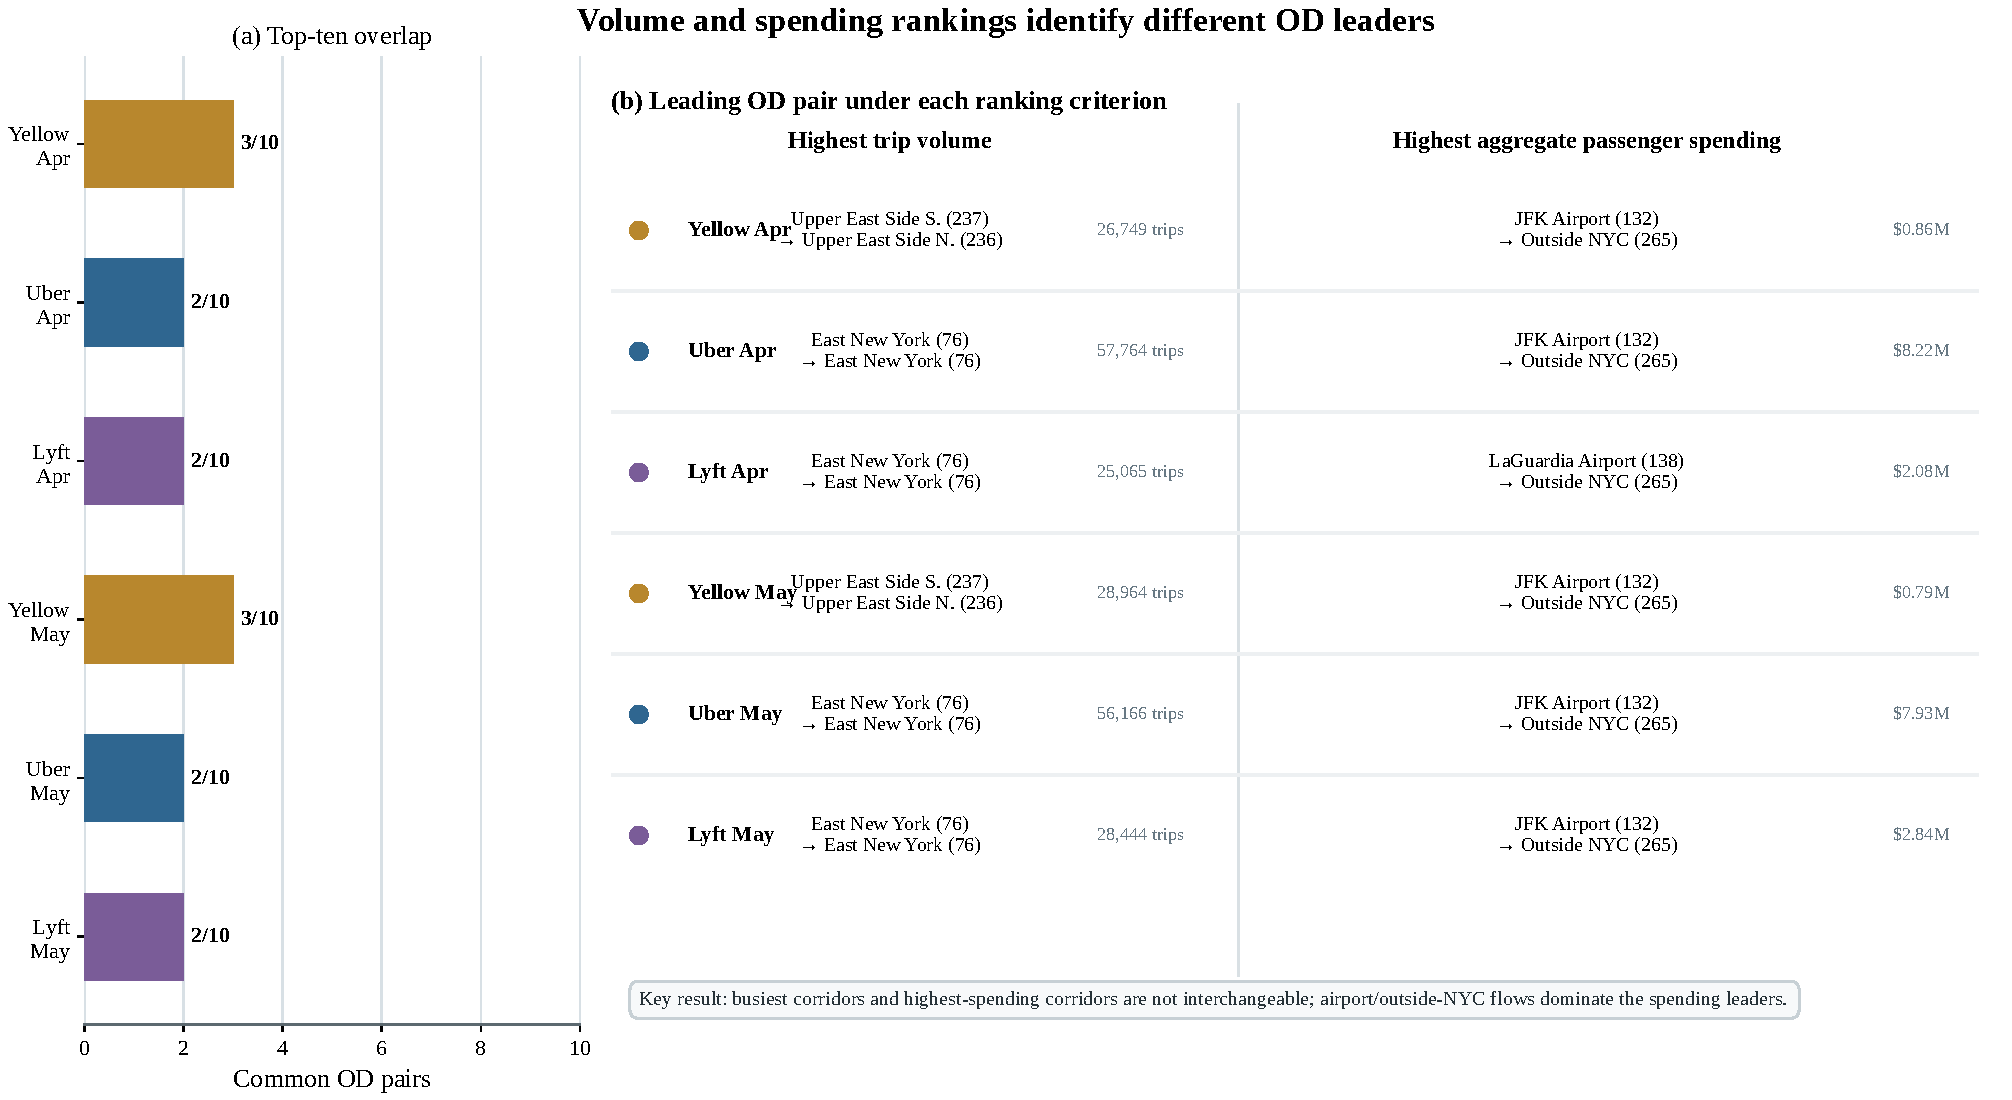
\includegraphics[width=.98\linewidth]{04_Results/paper_figures/main/fig4_od_ranking_summary.pdf}
\caption{\textbf{Trip volume and aggregate passenger spending identify different directed OD structures.} Panel (a) reports the overlap between the independently constructed top-ten volume and spending lists. Panel (b) names the leading OD pair under each criterion, making the contrast between high-frequency local flows and high-spending airport/outside-city flows explicit. Detailed top-ten OD-flow maps are provided in Appendix~\ref{app:spatial}; the eight required hotspot maps are included above in the main text.}
\label{fig:od}
\end{figure}
\FloatBarrier

\section{Task 3: Reported Ride-Pooling Activity}
\subsection{Method}
Let $n_{NN}$, $n_{YN}$, $n_{YY}$, and $n_{NY}$ denote the number of valid-status trips in the four request/match states and let
\[
V=n_{NN}+n_{YN}+n_{YY}+n_{NY}.
\]
Three distinct metrics are reported:
\begin{align}
\text{Pooling-request rate} &= \frac{n_{YN}+n_{YY}}{V},\\
\text{Reported matched rate} &= \frac{n_{NY}+n_{YY}}{V},\\
\text{Matching success among requests} &= \frac{n_{YY}}{n_{YN}+n_{YY}}.
\end{align}
The metrics are kept separate because they use different denominators and answer different questions. Zone-level matching success is reported only when at least 100 pooling requests are available, reducing instability from very small local samples.

\subsection{Results and interpretation}
Uber records substantially more pooling activity than Lyft. Its pooling-request rate decreases from 2.714\% in April to 2.532\% in May; its reported matched rate decreases from 1.661\% to 1.439\%; and matching success among requests decreases from 61.18\% to 56.82\%. Lyft request rates are only 0.0345\% and 0.0299\%, with matching success among requests of 3.77\% and 3.36\%. In April, Uber's pooling-request rate is approximately 79 times Lyft's; in May the ratio is approximately 85.

The distinction between request and match is important. A request rate describes participation in the platform's shared product, whereas matching success describes what fraction of those requests became reported matches. Figure~\ref{fig:pooling} therefore prints the actual percentages and separates the metrics into distinct panels rather than collapsing them into a single generic ``sharing rate.''

Zone-level comparisons use the assignment thresholds directly. Reported matched rates are shown only for zones with at least 100 valid-status trips, and matching success is shown only for zones with at least 100 pooling requests; below-threshold zones are treated as insufficient sample rather than zero. Uber has broad enough request volume for zone comparisons, with 232 April zones and 233 May zones meeting the 100-request threshold. The highest matching-success zones are Stuyvesant Heights in April (76.9\% of 5,173 requests) and Lower East Side in May (76.0\% of 4,618 requests). Lyft has too little request volume for stable zone-level interpretation: only three April zones and two May zones meet the 100-request threshold.

\begin{figure}[!htbp]
\centering
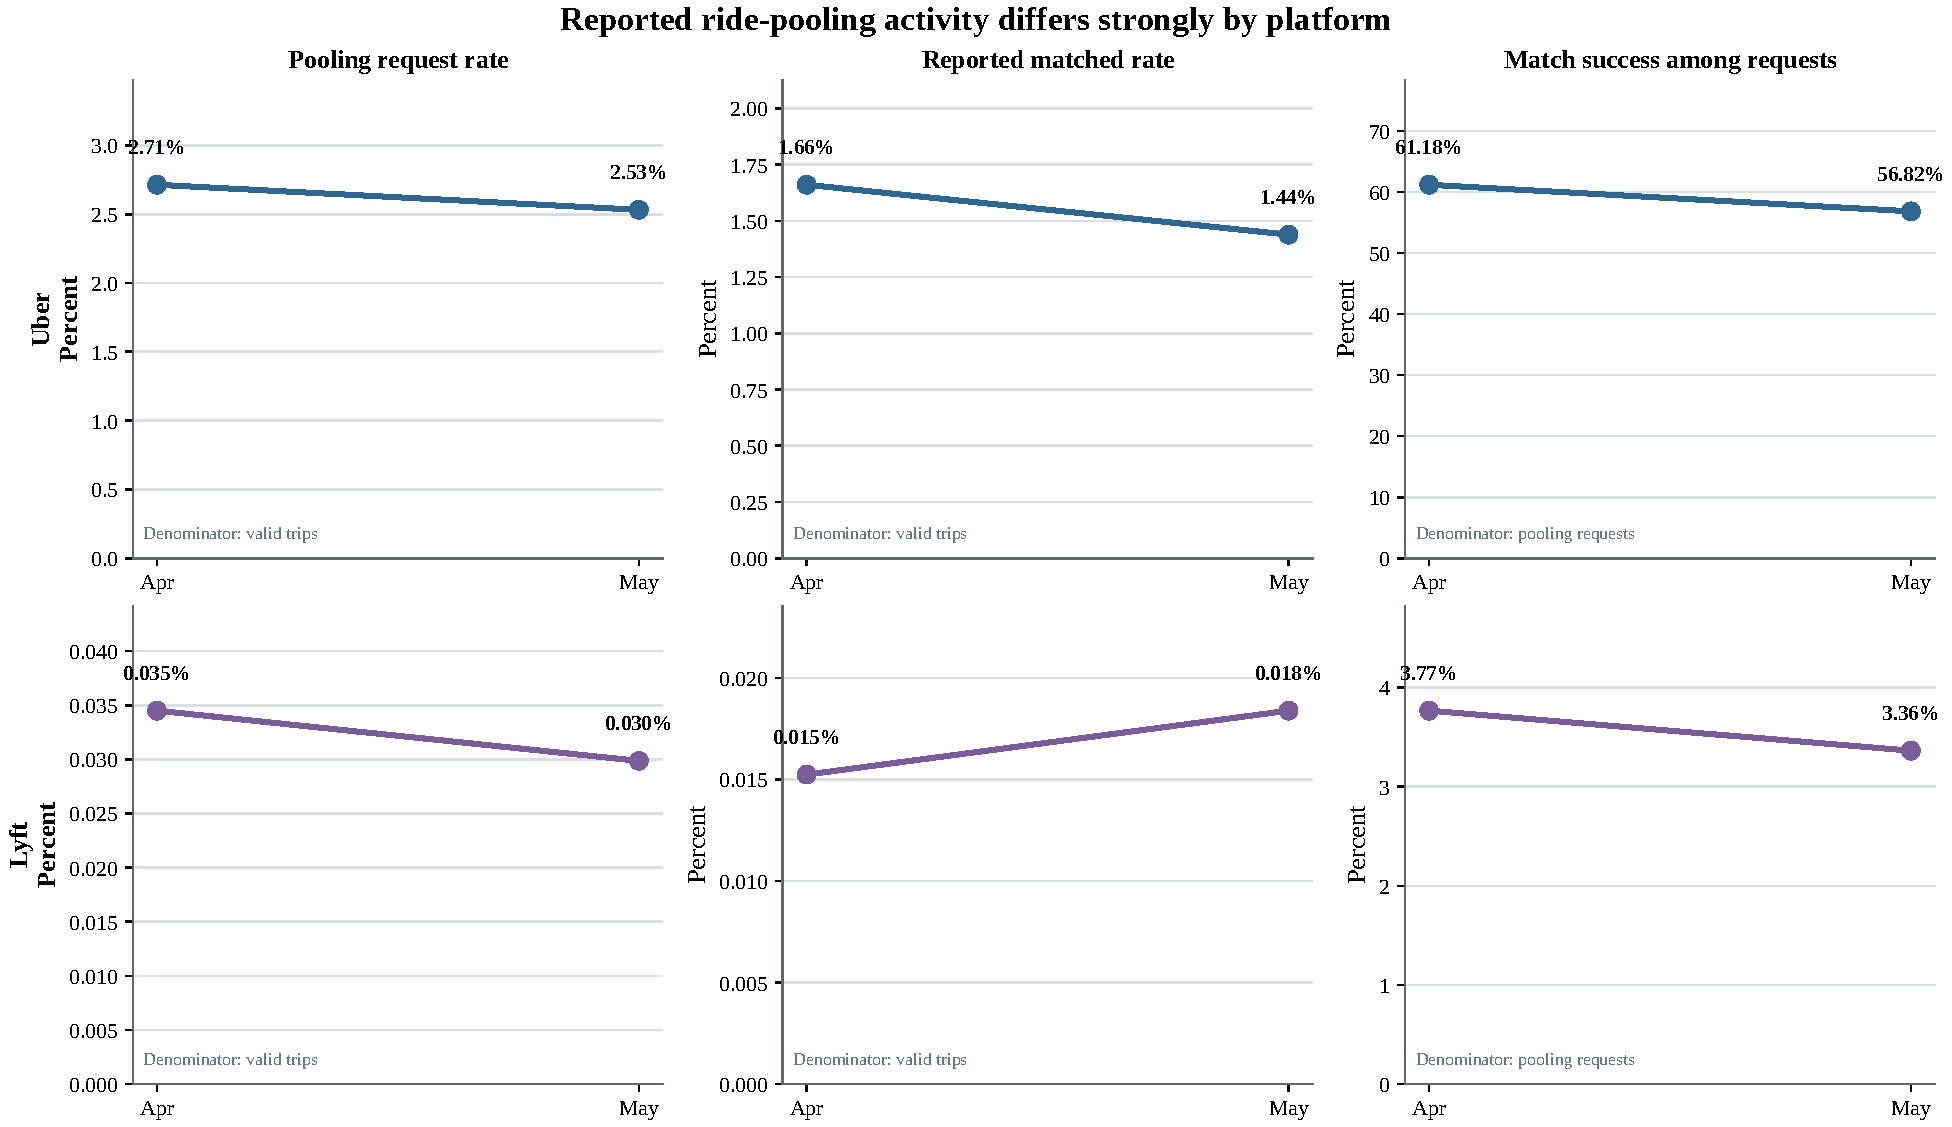
\includegraphics[width=.98\linewidth]{04_Results/paper_figures/main/fig5_pooling_metrics.pdf}
\caption{\textbf{Reported ride-pooling activity by platform and month.} The top row shows Uber and the bottom row Lyft. Columns separately report pooling requests per valid trip, reported matches per valid trip, and matching success among pooling requests. Numerical annotations should be used for cross-panel comparison because each panel has its own y-axis scale.}
\label{fig:pooling}
\end{figure}
\FloatBarrier

\section{Task 4: Observed Travel-Time Difference for Uber Shared Trips}
\subsection{Method}
Task 4 focuses on Uber because it provides essentially the entire usable \YY{} sample. Non-shared \NN{} trips form the reference population. A reference cell is defined by directed OD pair, pickup hour, and weekday/weekend category. April and May non-shared trips are pooled when constructing the reference, and a cell is used only when it contains at least 30 eligible \NN{} trips. The cell median travel time is used because recorded trip-time distributions are typically right-skewed.

For a supported shared trip $i$, let $T_i$ be its recorded trip time and $T_{\mathrm{ref},i}$ the median time of its matched non-shared cell. The observed absolute and relative differences are
\begin{align}
E_i &= T_i-T_{\mathrm{ref},i},\\
R_i &= 100\frac{T_i-T_{\mathrm{ref},i}}{T_{\mathrm{ref},i}}.
\end{align}
Negative values are retained. A shared trip without a sufficiently populated reference cell is not assigned a synthetic comparison. Instead, reference coverage is reported as part of the result.

\subsection{Monthly results}
In April, 121,673 of 255,383 eligible Uber \YY{} trips are supported, giving 47.64\% coverage. Their median observed shared-minus-reference travel-time difference is +4.53 min, with an interquartile range of 0.25--10.01 min. In May, 110,559 of 220,904 eligible shared trips are supported (50.05\% coverage), and the median difference is +4.98 min with an interquartile range of 0.71--10.48 min. Median relative differences are 25.83\% and 29.35\%, respectively.

Two aspects should be read together. First, the median supported shared trip has a longer recorded travel time than the median non-shared trip in the same OD--hour--day-type cell. Second, only about half of the eligible shared trips have a sufficiently populated reference. The result therefore characterizes the supported subset rather than the complete Uber shared-trip population.

\begin{figure}[!htbp]
\centering
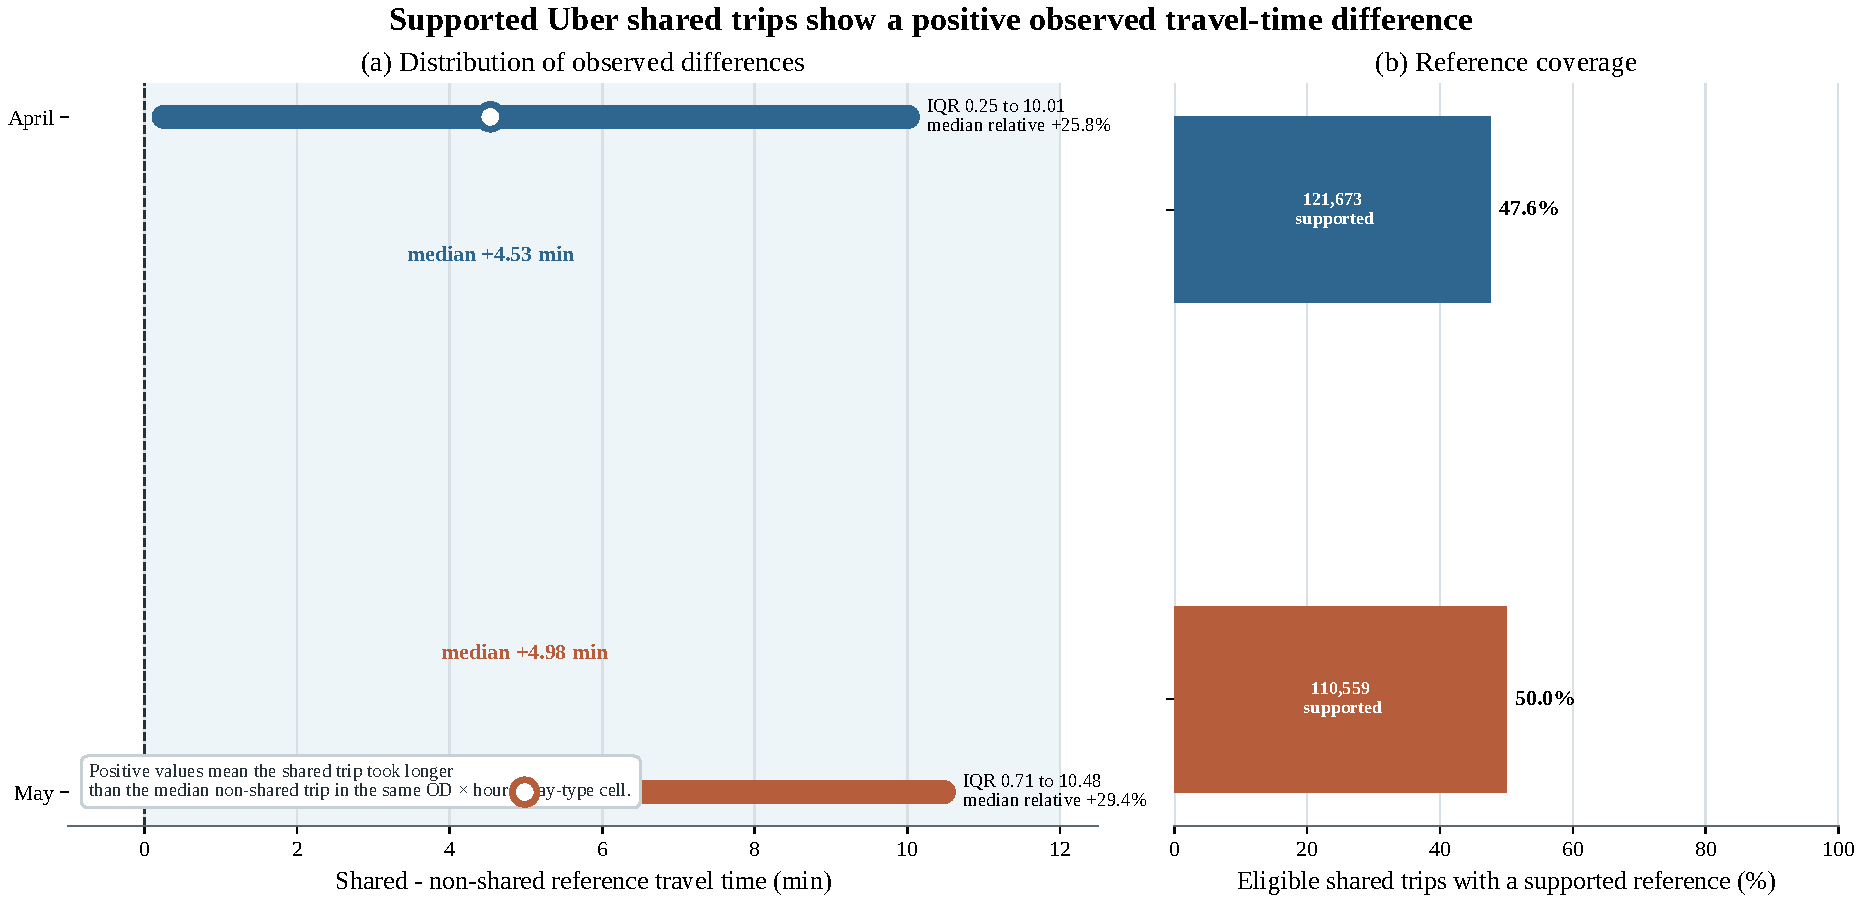
\includegraphics[width=.98\linewidth]{04_Results/paper_figures/main/fig6_travel_time_monthly.pdf}
\caption{\textbf{Monthly observed travel-time differences for supported Uber shared trips.} Panel (a) shows the interquartile range and median of $E_i=T_i-T_{\mathrm{ref},i}$; positive values indicate a longer recorded travel time than the non-shared cell median. Panel (b) gives reference coverage and the supported/eligible sample counts. The approximately +4.5 to +5.0 min medians should therefore be interpreted together with the 47.6--50.0\% coverage.}
\label{fig:traveltime}
\end{figure}

\subsection{Hourly pattern and coverage}
Hourly medians vary less than reference coverage. In April, the lowest hourly median is 3.69 min at 10:00 and the highest is 5.05 min at 07:00. In May, the range is 4.12 min at 04:00 to 5.62 min at 17:00. Coverage falls sharply during some early-morning periods; the May 04:00 comparison, for example, has only 23.87\% support. This is why the hourly difference should not be interpreted independently of the coverage curve.

The within-zone and between-zone split shows that most supported shared trips are between-zone trips. Between-zone \YY{} trips have median $E=4.86$ min and median $R=27.4\%$ among 226,297 supported trips, with 48.1\% reference coverage. Within-zone \YY{} trips have a smaller median absolute excess of 2.00 min but a larger median relative excess of 31.4\% among 5,935 supported trips, with 98.7\% reference coverage. Geographic zone summaries are therefore trip-weighted means over supported trips, not equal-weighted OD-cell averages.

\begin{figure}[!htbp]
\centering
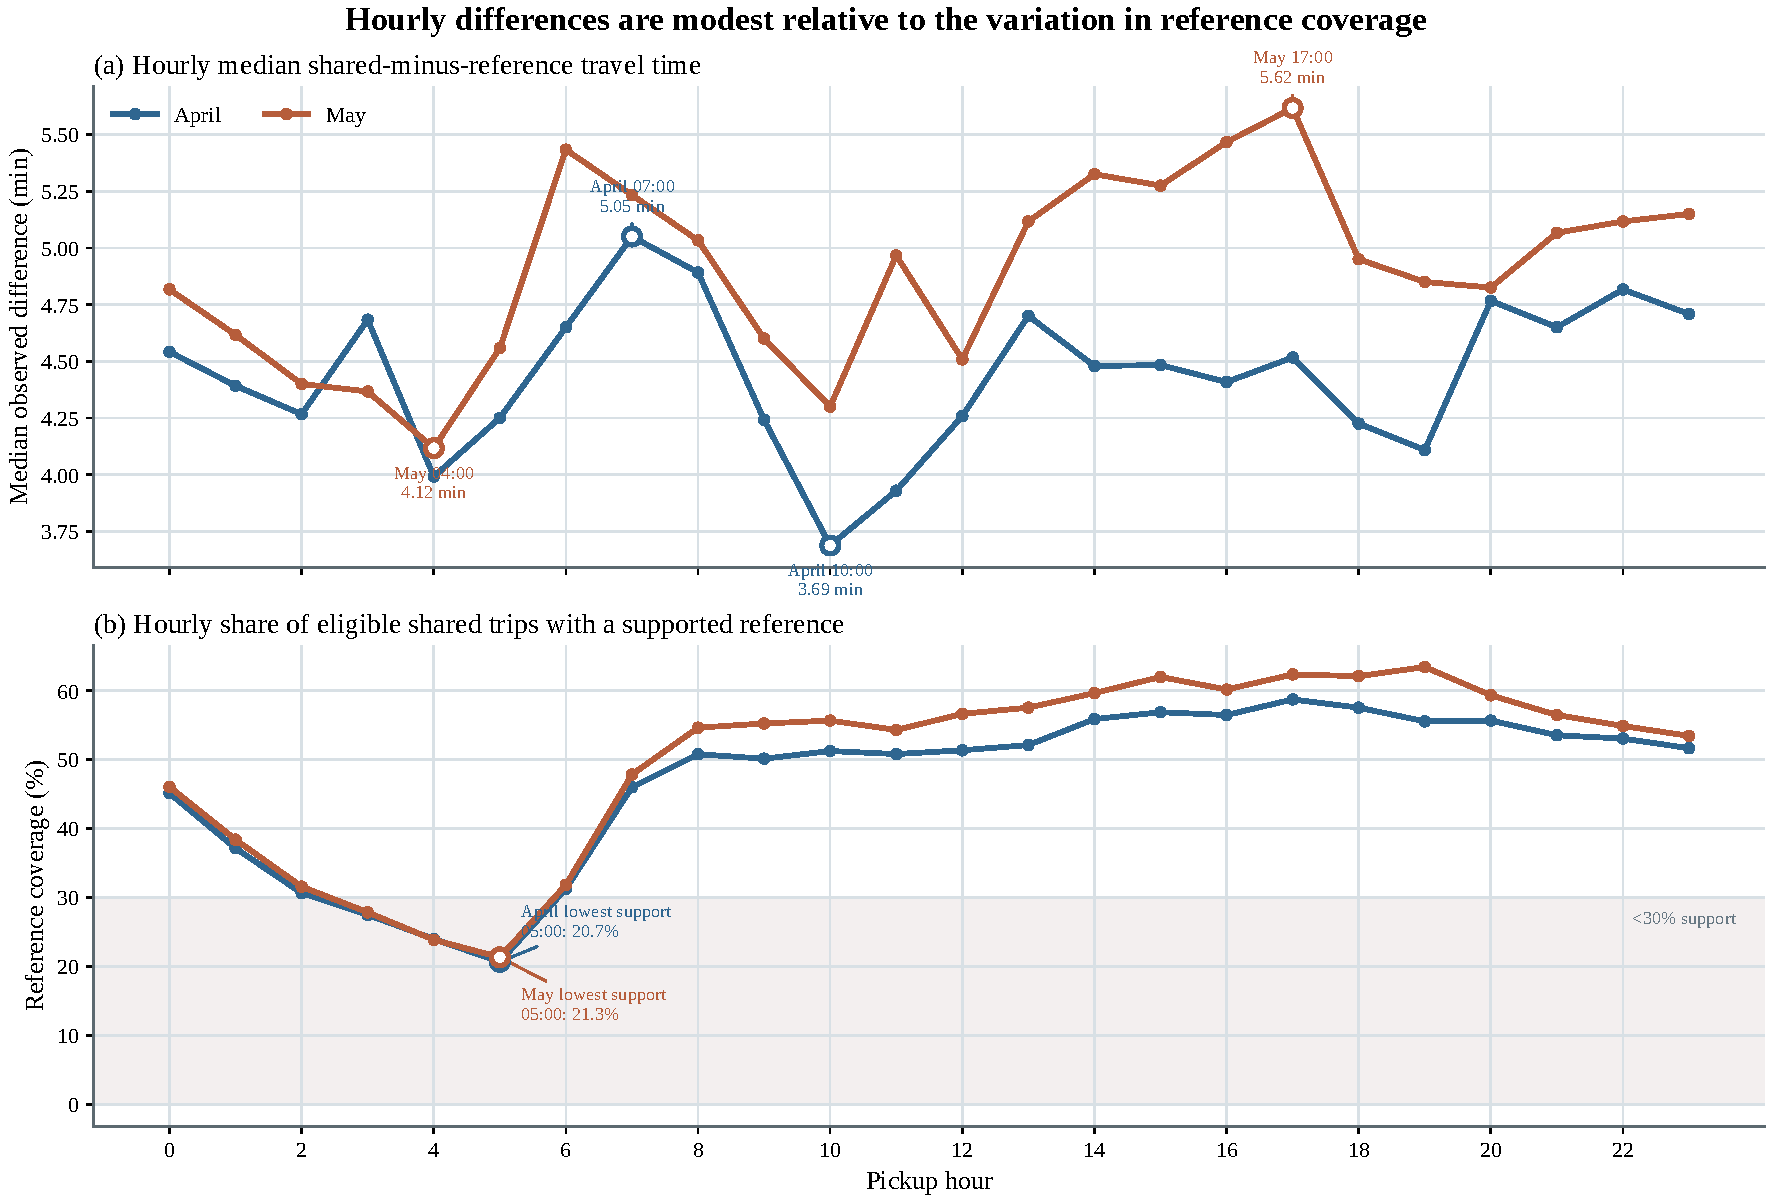
\includegraphics[width=.98\linewidth]{04_Results/paper_figures/main/fig7_travel_time_hourly.pdf}
\caption{\textbf{Hourly travel-time pattern and reference coverage.} Panel (a) plots the hourly median observed travel-time difference and annotates the within-month minima and maxima. Panel (b) plots the corresponding support rate and highlights coverage below 30\%. The travel-time curve changes moderately through the day, whereas reference support varies more strongly.}
\label{fig:hourly}
\end{figure}

The Task 4 comparison is observational rather than causal. OD--hour--day-type matching does not control exact endpoints, contemporaneous congestion, route choice, passenger selection, or the actual distance/time over which two passengers shared a vehicle. The reference median is therefore a transparent benchmark, not a counterfactual travel time or an estimate of causal pooling delay.
\FloatBarrier

\section{Task 5: Observed Passenger-Spending Difference}
\subsection{Method}
Reported \YY{} trips are compared with \NN{} trips within the same company, pickup month, directed OD pair, pickup hour, and weekday/weekend category. A non-shared reference cell must contain at least 30 trips. For each supported shared trip, passenger spending is compared with the mean spending of its non-shared cell. If $S_i$ is shared-trip spending and $\bar N_{c(i)}$ is the mean non-shared spending in cell $c(i)$, the estimator is
\[
\hat\Delta = \frac{1}{n}\sum_{i=1}^{n}\left(S_i-\bar N_{c(i)}\right).
\]
Negative values indicate lower observed passenger spending for supported shared trips. Confidence intervals use standard errors clustered by pickup date to account for same-day dependence among matched differences.

\subsection{Results and interpretation}
For Uber, 85,060 April shared trips have a supported spending reference (33.31\% coverage), with a mean shared-minus-reference difference of -\usd8.20 and a 95\% confidence interval of -\usd8.85 to -\usd7.55. In May, 77,449 shared trips are supported (35.06\% coverage), with a mean difference of -\usd8.14 and a 95\% confidence interval of -\usd8.95 to -\usd7.33. Relative to the matched reference means, these correspond to approximately -28.4\% and -28.7\%.

Lyft's supported estimates are more negative (-\usd16.26 in April and -\usd20.85 in May), but they rely on only 47 and 38 supported shared trips. The Lyft intervals and tiny sample sizes therefore make those estimates substantially less stable than the Uber results. Figure~\ref{fig:spending} places the point estimate, confidence interval, sample size, and coverage together so the magnitude is not read without its data support.

\begin{figure}[!htbp]
\centering
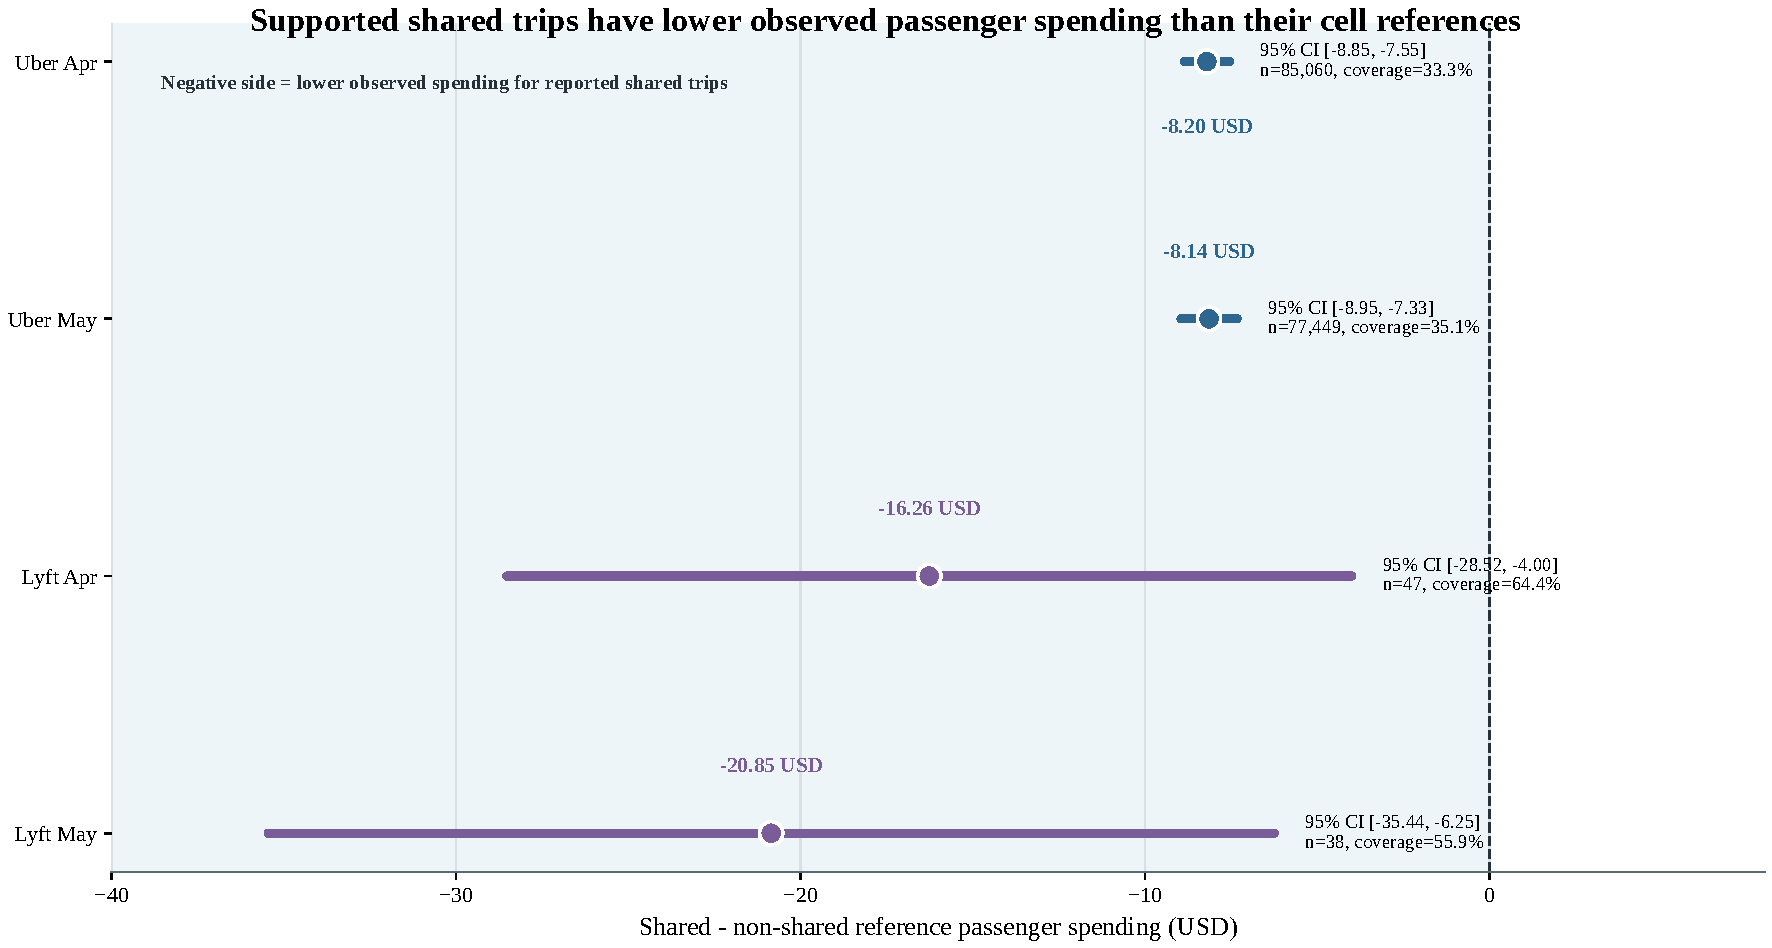
\includegraphics[width=.98\linewidth]{04_Results/paper_figures/main/fig8_spending_difference.pdf}
\caption{\textbf{Observed passenger-spending differences in supported comparison cells.} Points show the mean shared-minus-reference spending difference and horizontal segments show date-clustered 95\% confidence intervals. Negative values indicate lower observed spending for reported shared trips. Uber estimates are close to -\usd8 in both months with tens of thousands of supported trips; Lyft estimates are based on only 47 and 38 trips.}
\label{fig:spending}
\end{figure}

As in Task 4, this is a descriptive comparison rather than a causal estimate. Matching controls for coarse spatial and temporal context but not exact endpoints, route choice, passenger selection, dynamic pricing, promotions, or the true overlap period of pooled passengers. Task 5.2, concerning potential matches among non-shared trips, is not analysed here and no bonus credit is claimed.
\FloatBarrier

\section{Overall Discussion}
The five tasks together show why the definition of each denominator and comparison population matters. The spatial analysis indicates that service demand, trip frequency, and aggregate passenger spending identify different aspects of the urban mobility system. Yellow Taxi activity remains strongly concentrated in Manhattan, whereas HVFHV activity is broader and includes prominent airport/outside-city flows. The small overlap between high-volume and high-spending OD rankings demonstrates that a single ranking criterion cannot summarize both operational demand and monetary importance.

The pooling analysis also shows that the available matched shared-trip population is highly platform dependent. Uber has a much larger request rate and much higher matching success than Lyft, so the effective sample for later shared-trip comparisons is overwhelmingly Uber. This limitation is visible before any travel-time or spending estimator is computed and should constrain how broadly the Task 4 and Task 5 findings are generalized.

For the supported Uber sample, Task 4 and Task 5 point in different directions on different outcomes: recorded travel time is higher relative to the matched non-shared reference, while recorded passenger spending is lower. This pattern is consistent with a descriptive time--cost trade-off, but the design does not establish that pooling itself caused either difference. Reference coverage is therefore part of the evidence, not a secondary diagnostic: about half of eligible Uber \YY{} trips are represented in Task 4 and about one third in Task 5.

Several data limitations remain. TLC notes that the records are provider-submitted and are not guaranteed to be error-free \cite{tlc_tripdata}. The request and match variables indicate recorded status but do not identify the matched passenger, the duration of shared occupancy, or the true shared segment of the trip. Taxi Zones are coarse spatial units rather than exact endpoints, and zone 265 has no polygon. Finally, the two-month study period provides a detailed short-run snapshot rather than evidence about seasonality or long-term change.

\section{Conclusion}
This assignment analyses more than 50.9 million April--May 2026 Yellow Taxi and HVFHV trip records through five linked tasks. Task 1 establishes the retained sample and shows that usable reported matched shared trips are overwhelmingly Uber. Task 2 finds persistent service-specific spatial patterns and demonstrates that high-volume OD pairs differ substantially from high-spending OD pairs. Task 3 shows that Uber records much higher pooling-request and matching-success rates than Lyft. Task 4 finds median observed Uber shared-minus-reference travel-time differences of +4.53 min in April and +4.98 min in May among supported trips, with coverage close to 50\%. Task 5 finds mean observed Uber shared-minus-reference passenger-spending differences of about -\usd8 in both months, with coverage near one third. The main analytical lesson is that the point estimate, denominator, matching rule, and reference coverage should be reported together. The travel-time and spending results are conditional observational comparisons and should not be interpreted as causal effects of ride pooling.

\begin{thebibliography}{9}
\bibitem{tlc_tripdata}
New York City Taxi and Limousine Commission, ``TLC Trip Record Data,'' 2026. Available: \url{https://www.nyc.gov/site/tlc/about/tlc-trip-record-data.page}. Accessed: Oct. 3, 2026.

\bibitem{tlc_hvfhv}
New York City Taxi and Limousine Commission, ``Data Dictionary -- High Volume FHV Trip Records,'' Mar. 18, 2025. Available: \url{https://www.nyc.gov/assets/tlc/downloads/pdf/data_dictionary_trip_records_hvfhs.pdf}.

\bibitem{tlc_zoneguide}
New York City Taxi and Limousine Commission, ``Trip Record User Guide: Taxi Zone Maps and Lookup Tables,'' available via the TLC Trip Record Data documentation. Available: \url{https://www.nyc.gov/assets/tlc/downloads/pdf/trip_record_user_guide.pdf}.
\end{thebibliography}

\appendix
\section{Supplementary Spatial Results}
\label{app:spatial}
The appendix contains the detailed OD-flow rankings and zone-level diagnostics supporting Tasks 2--4. The eight required Task 2.1 hotspot maps are included in the main text in Figures~\ref{fig:spatial_apr} and \ref{fig:spatial_may}. OD arrows connect Taxi Zone centroids and should not be interpreted as driven routes. Zone 265 (Outside of NYC) is retained in ranked lists but has no drawable polygon. Gray areas in zone-level pooling maps indicate insufficient sample rather than a zero rate.
\begingroup
\captionsetup{font=footnotesize,skip=3pt,hypcap=false}
\setlength{\abovecaptionskip}{3pt}
\setlength{\belowcaptionskip}{0pt}

\subsection{Detailed directed OD rankings}
The following compact pages show the ten leading directed OD pairs by trip volume and by aggregate passenger spending for each service and month. The original map images are unchanged; only their placement in the supplement is condensed.

\begin{center}
\centering
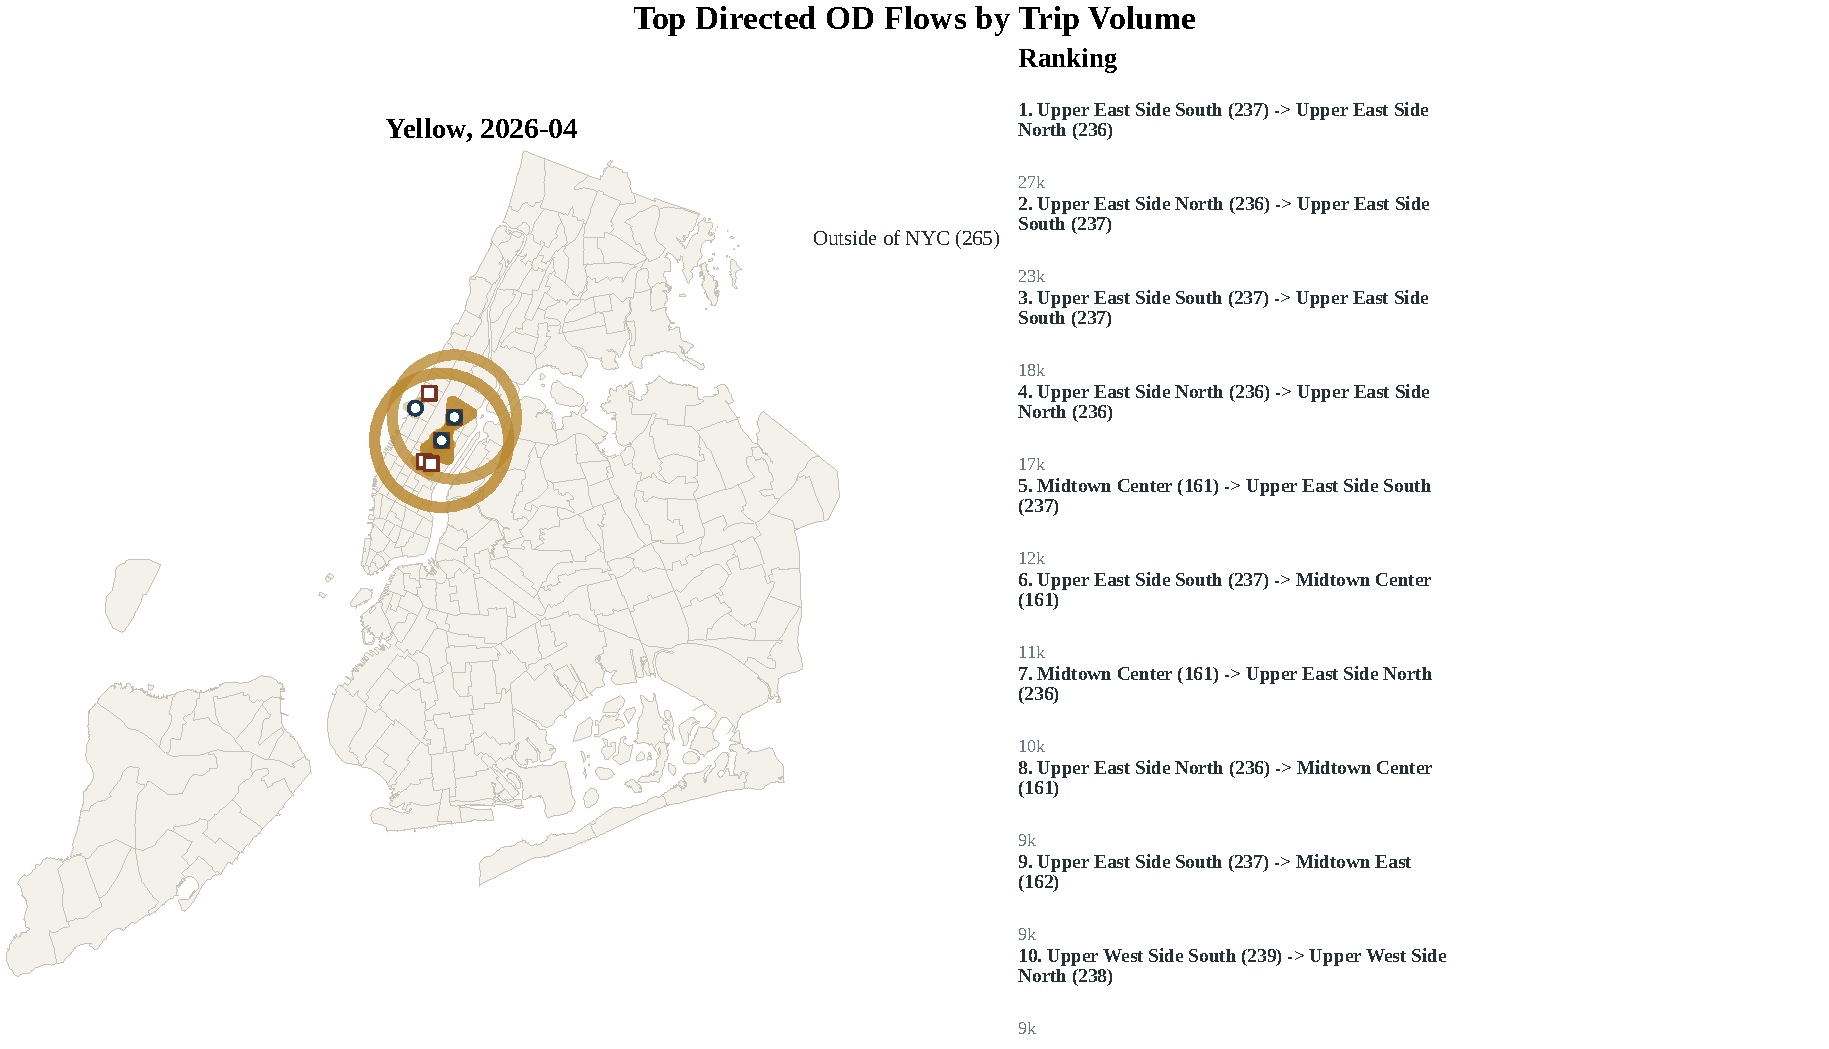
\includegraphics[height=.265\textheight,width=.98\linewidth,keepaspectratio]{04_Results/report_figures/appendix/task2_od_volume_2026-04_yellow.pdf}\par\vspace{0.2em}
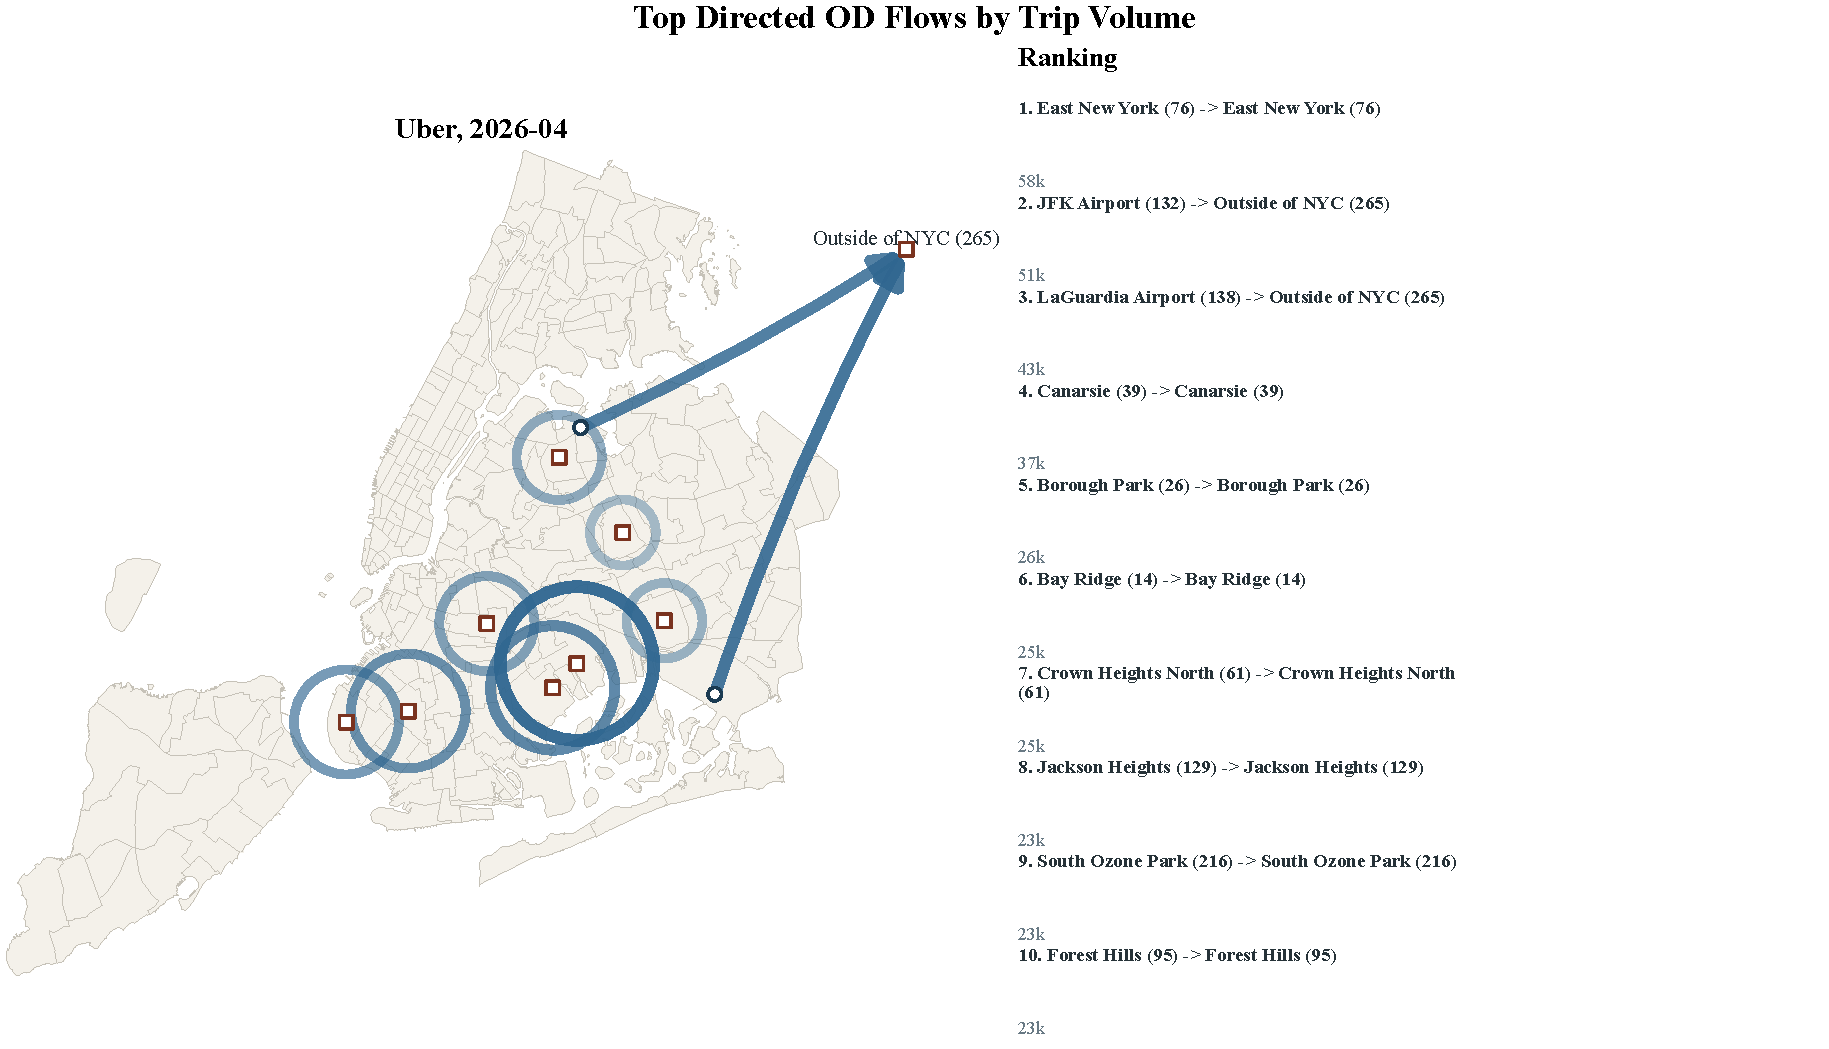
\includegraphics[height=.265\textheight,width=.98\linewidth,keepaspectratio]{04_Results/report_figures/appendix/task2_od_volume_2026-04_uber.pdf}\par\vspace{0.2em}
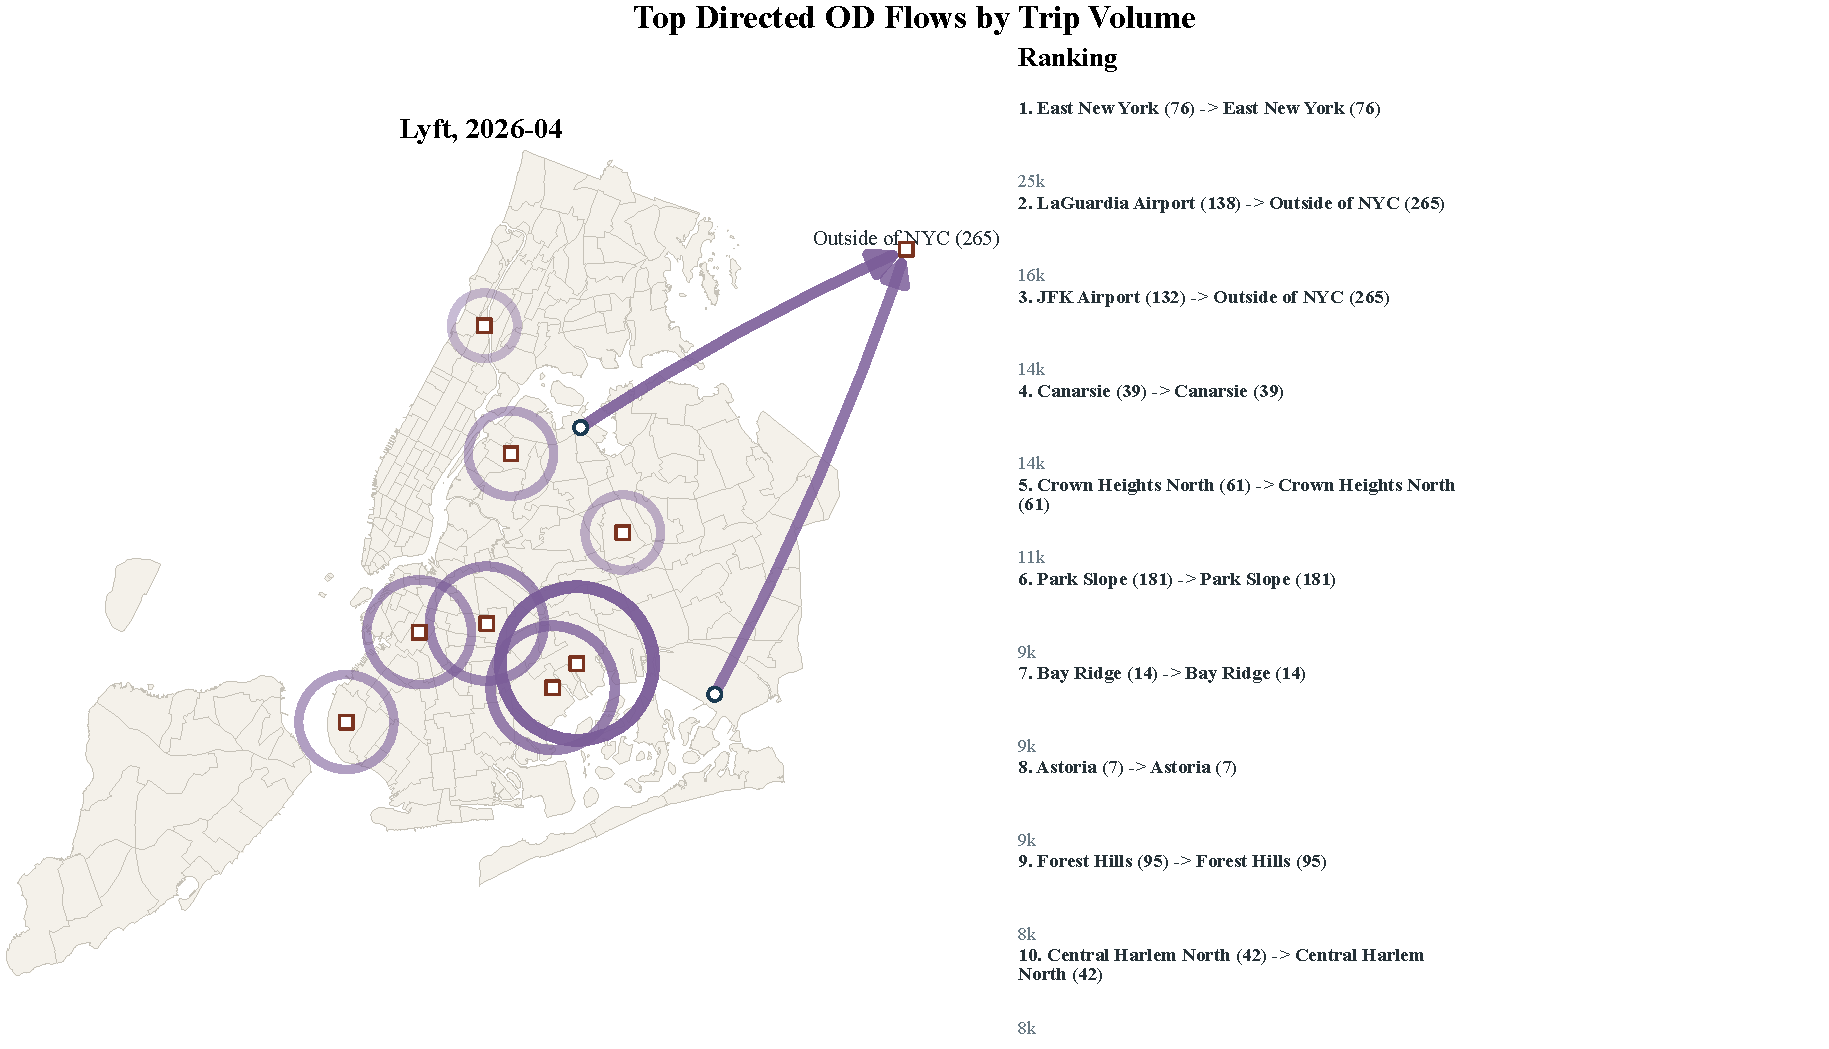
\includegraphics[height=.265\textheight,width=.98\linewidth,keepaspectratio]{04_Results/report_figures/appendix/task2_od_volume_2026-04_lyft.pdf}
\captionof{figure}{Top ten OD flows by trip volume, 2026-04. Panels from top to bottom: Yellow Taxi, Uber, and Lyft.}
\end{center}
\clearpage

\begin{center}
\centering
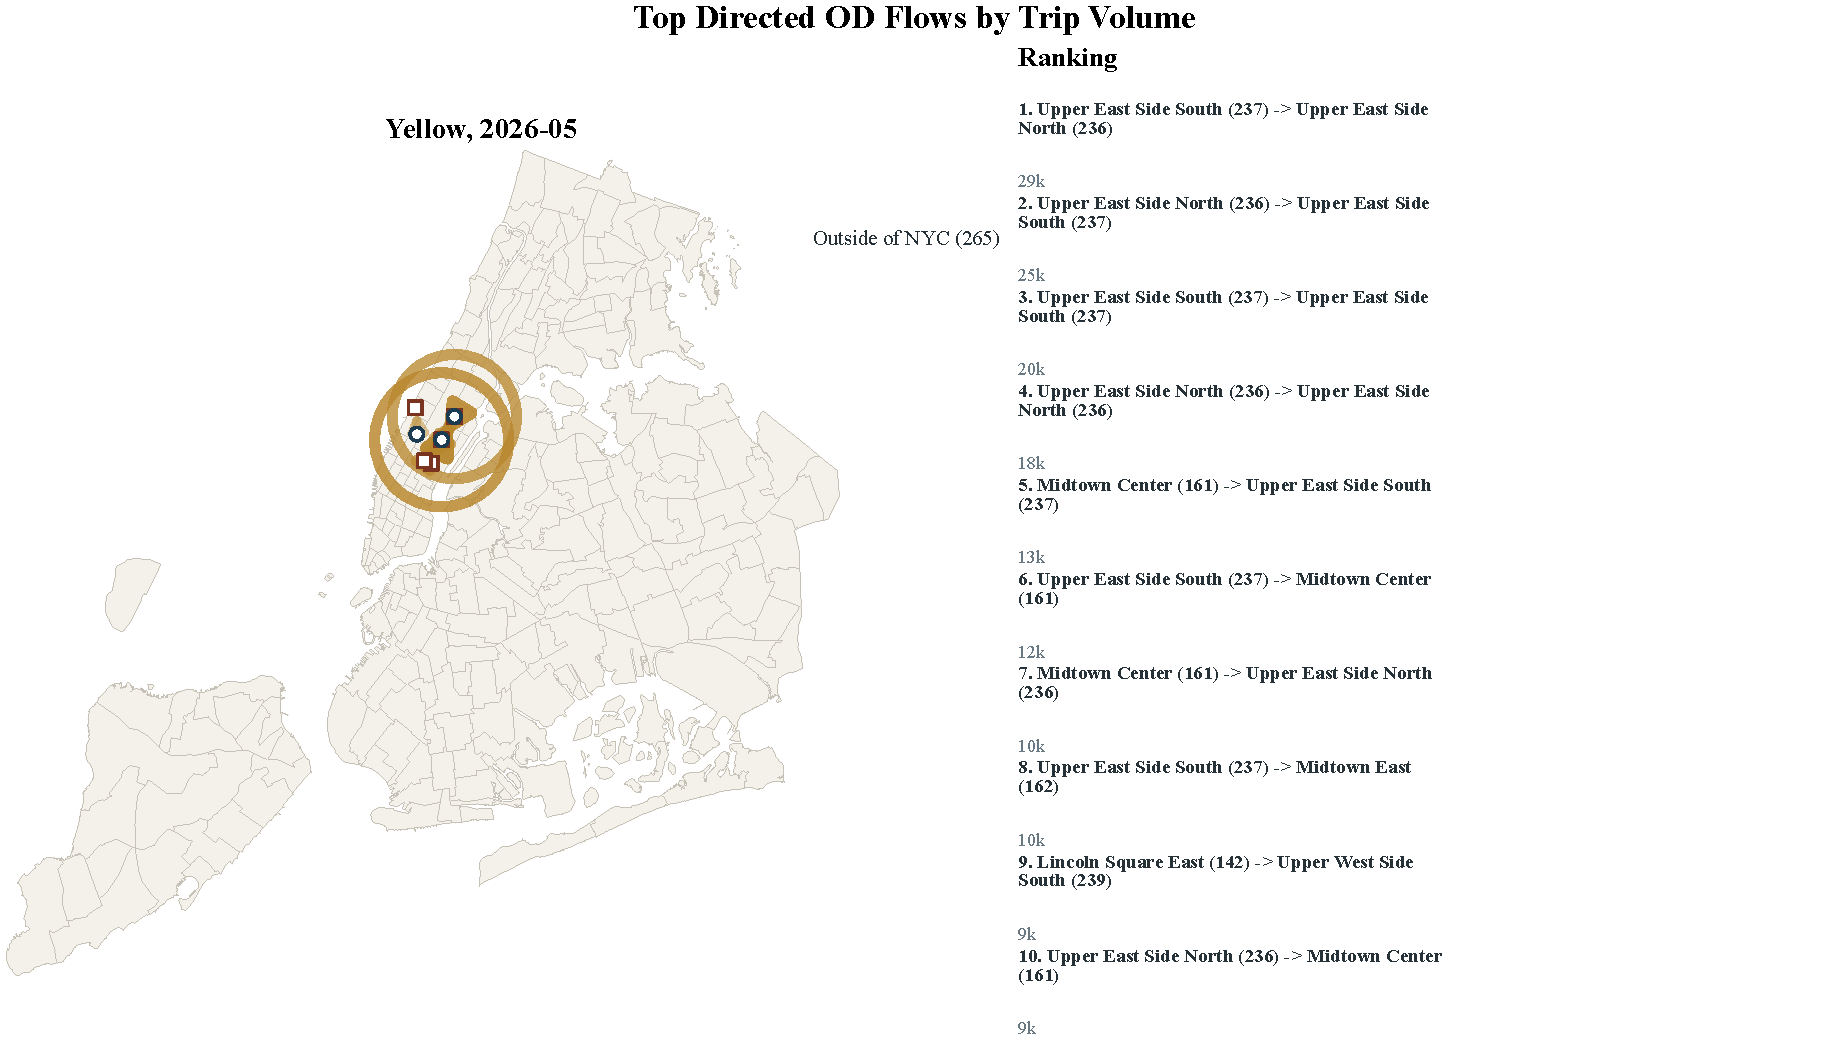
\includegraphics[height=.265\textheight,width=.98\linewidth,keepaspectratio]{04_Results/report_figures/appendix/task2_od_volume_2026-05_yellow.pdf}\par\vspace{0.2em}
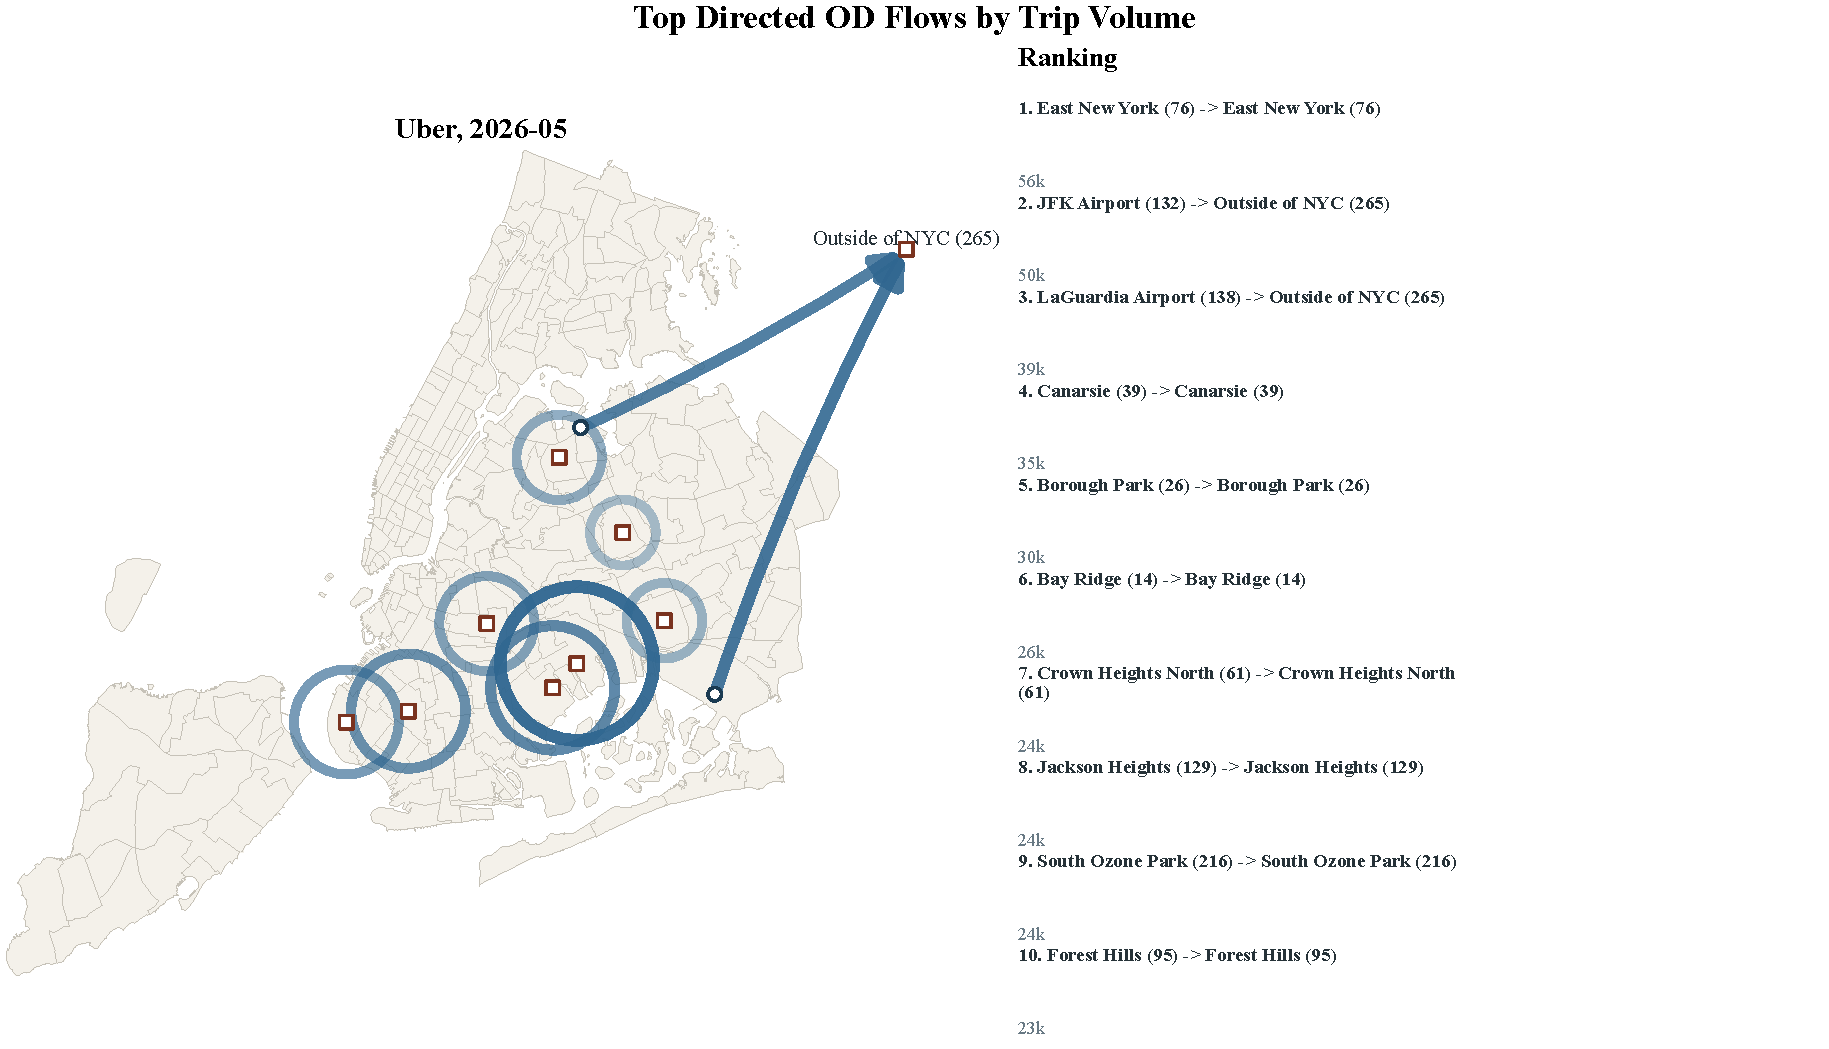
\includegraphics[height=.265\textheight,width=.98\linewidth,keepaspectratio]{04_Results/report_figures/appendix/task2_od_volume_2026-05_uber.pdf}\par\vspace{0.2em}
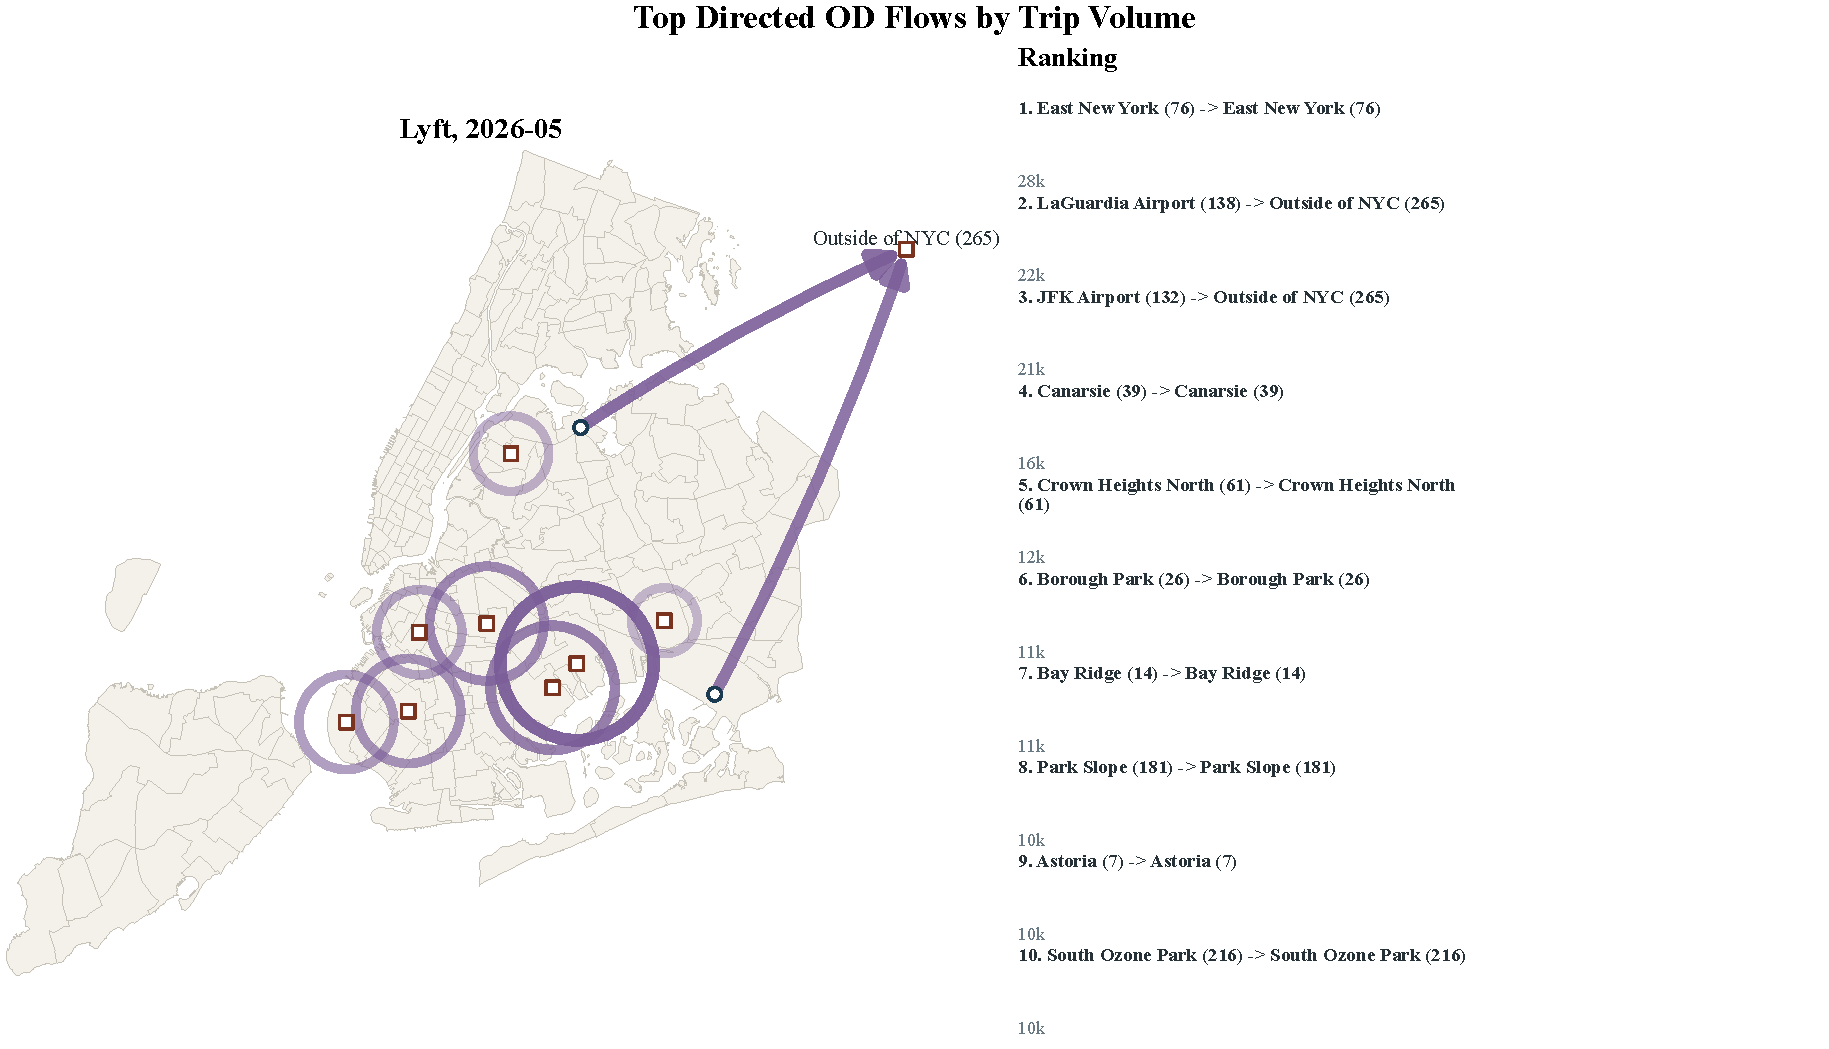
\includegraphics[height=.265\textheight,width=.98\linewidth,keepaspectratio]{04_Results/report_figures/appendix/task2_od_volume_2026-05_lyft.pdf}
\captionof{figure}{Top ten OD flows by trip volume, 2026-05. Panels from top to bottom: Yellow Taxi, Uber, and Lyft.}
\end{center}
\clearpage

\begin{center}
\centering
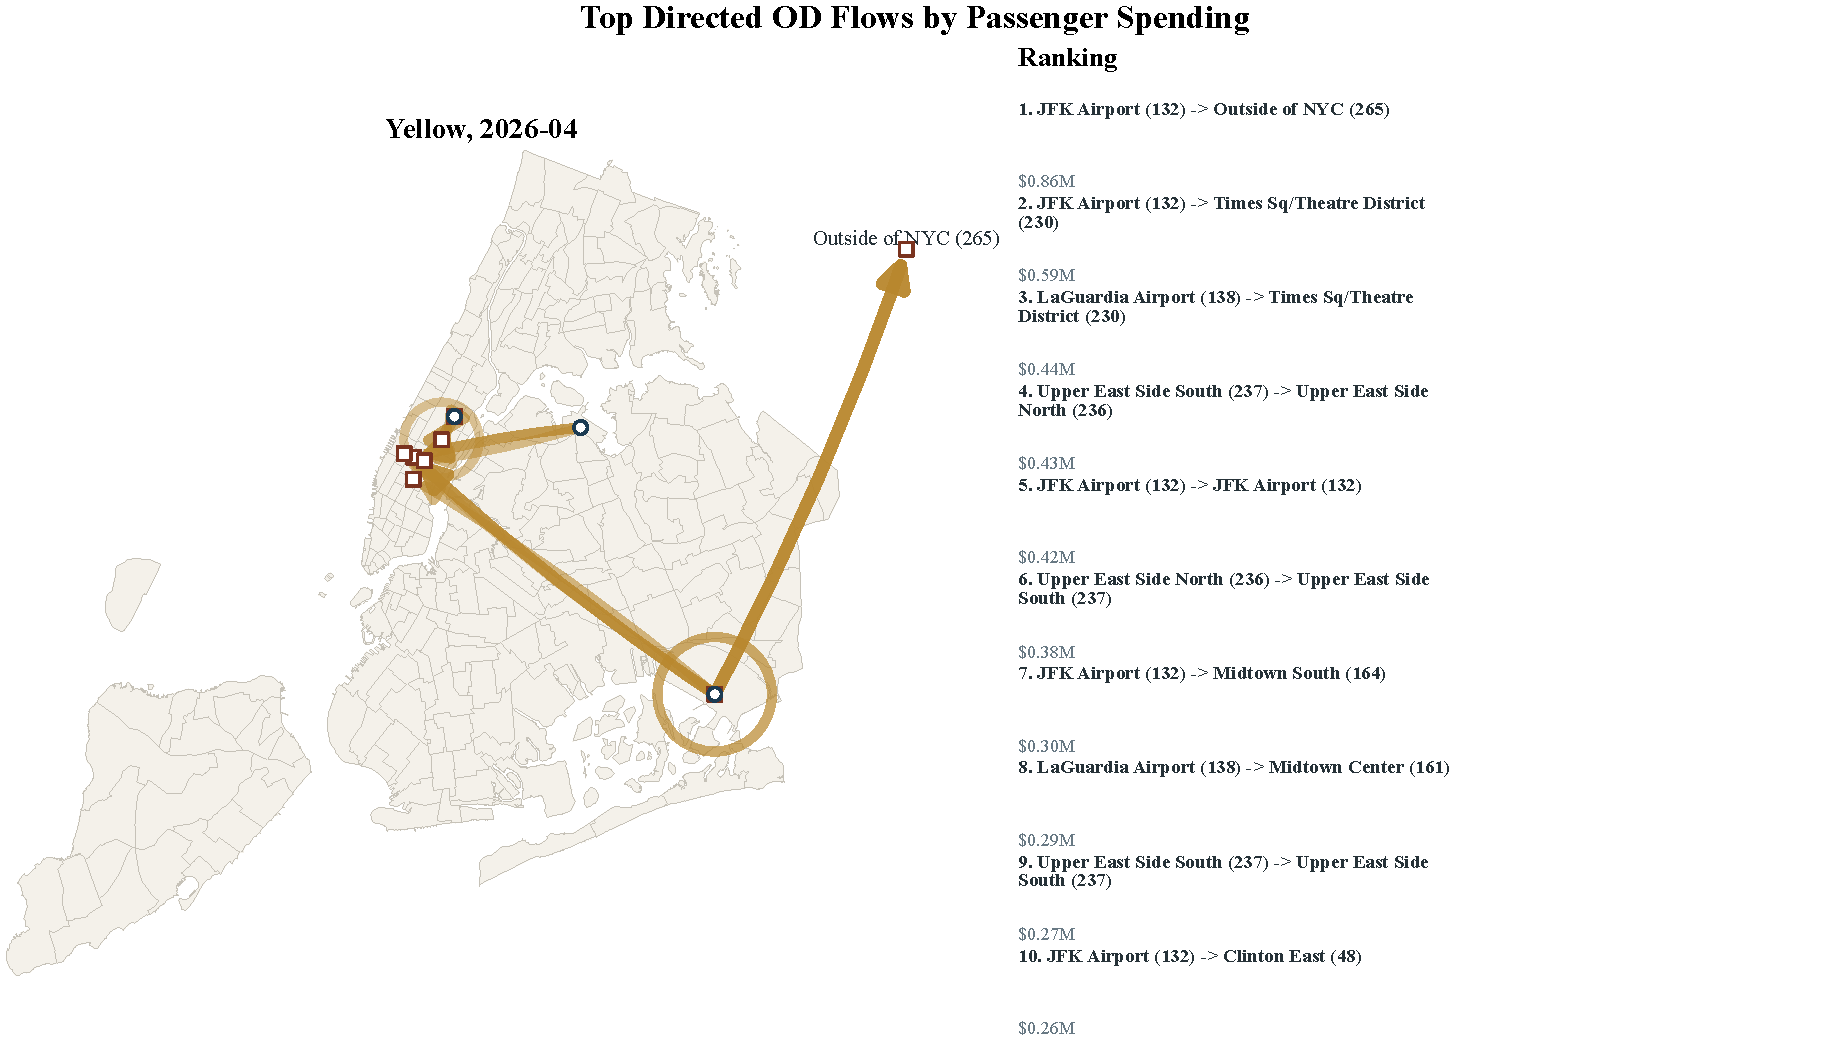
\includegraphics[height=.265\textheight,width=.98\linewidth,keepaspectratio]{04_Results/report_figures/appendix/task2_od_spending_2026-04_yellow.pdf}\par\vspace{0.2em}
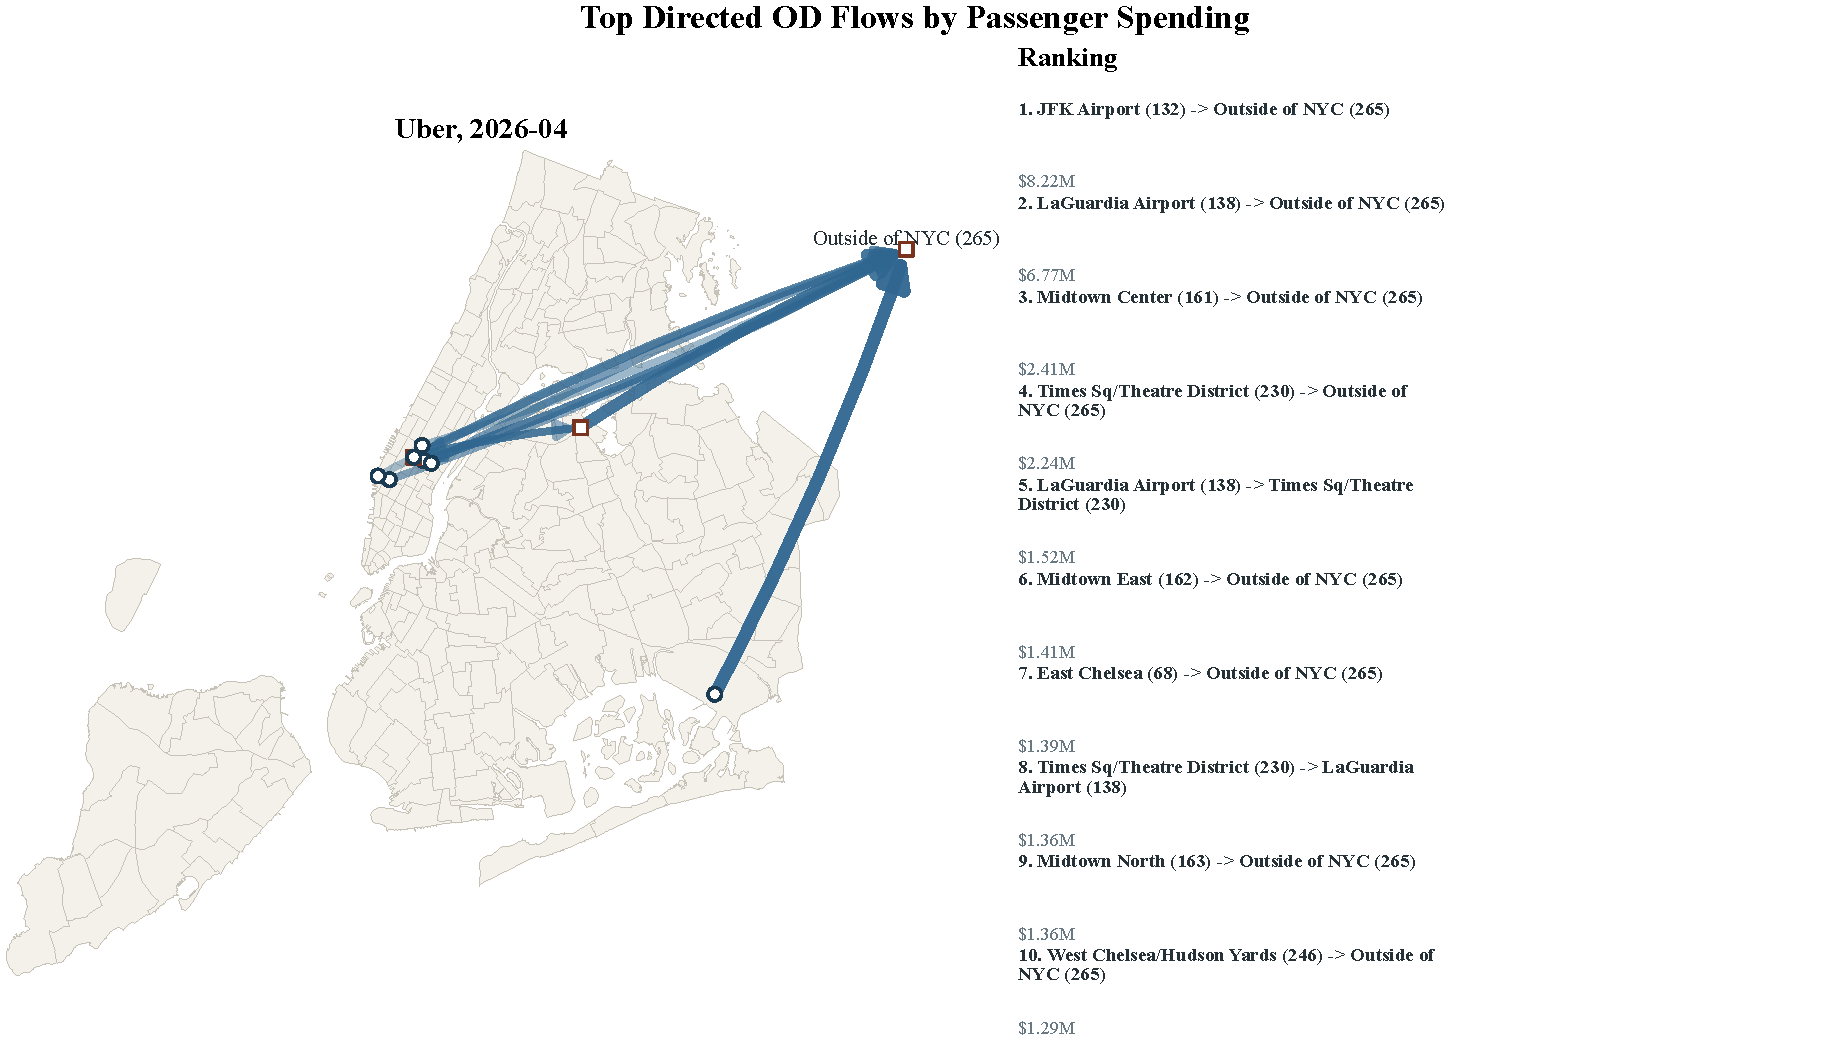
\includegraphics[height=.265\textheight,width=.98\linewidth,keepaspectratio]{04_Results/report_figures/appendix/task2_od_spending_2026-04_uber.pdf}\par\vspace{0.2em}
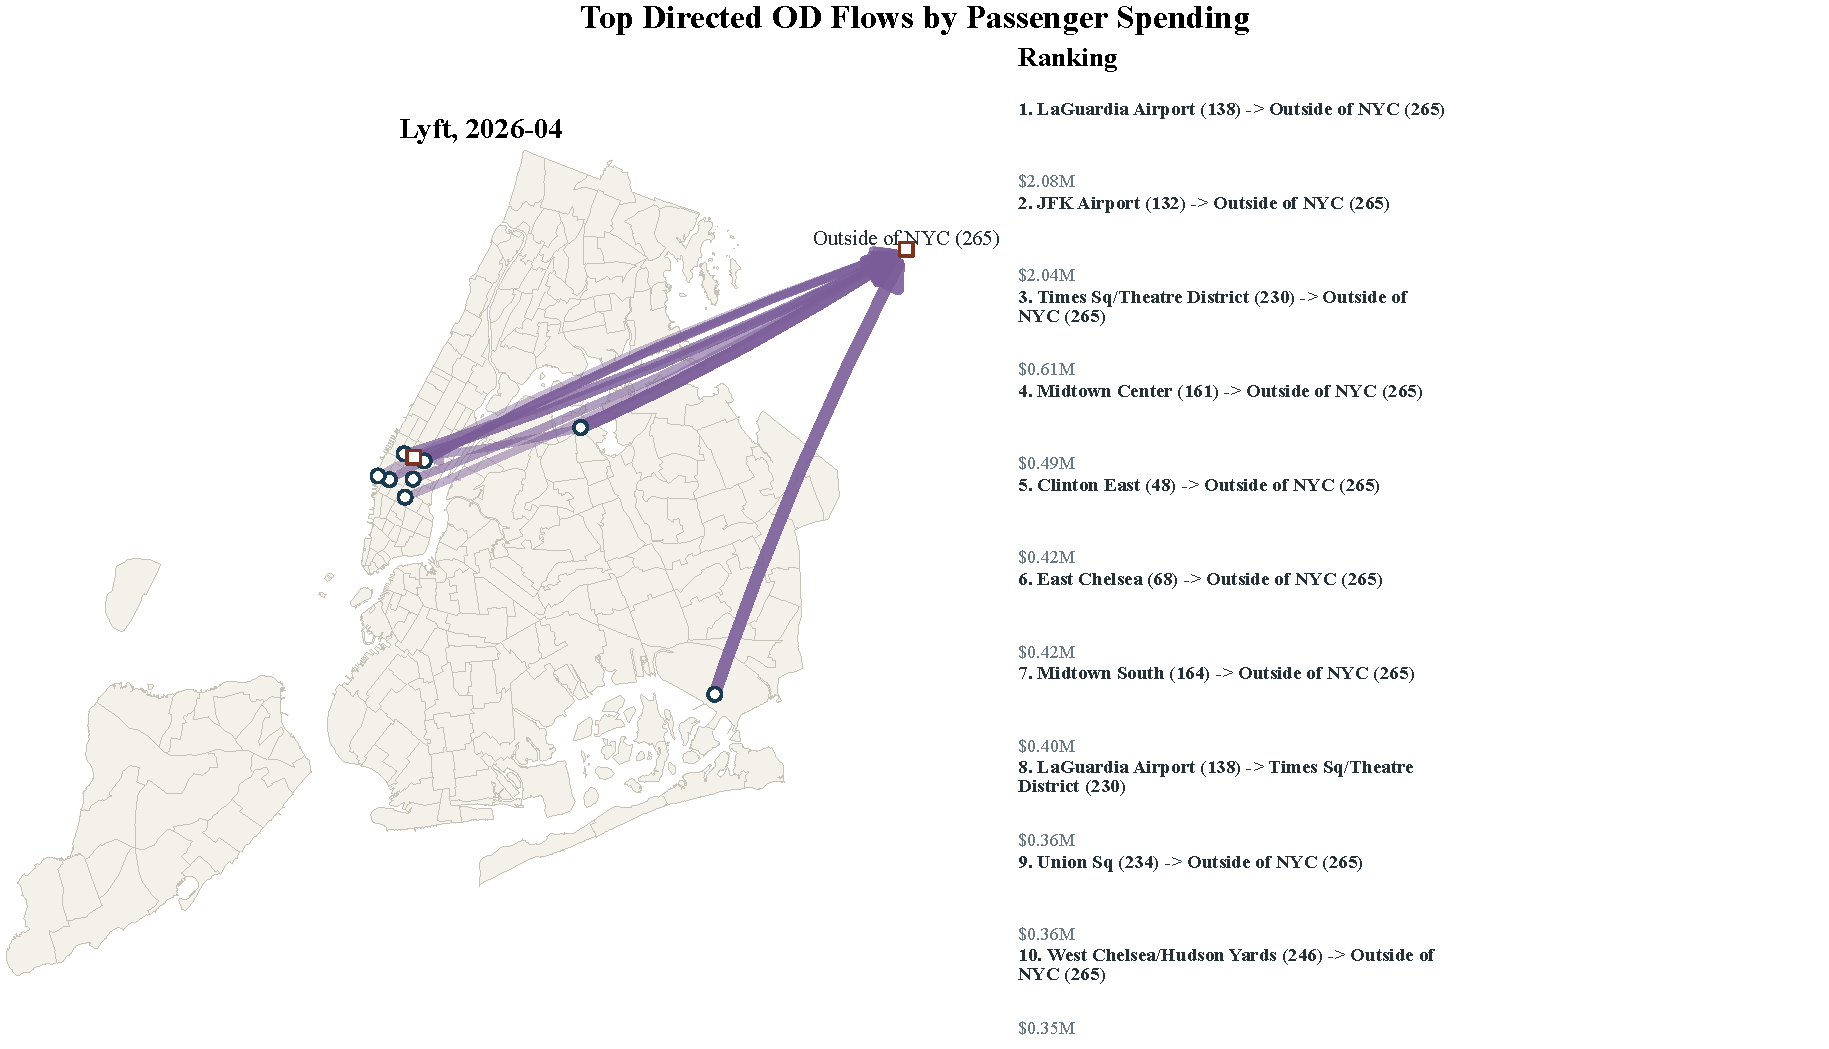
\includegraphics[height=.265\textheight,width=.98\linewidth,keepaspectratio]{04_Results/report_figures/appendix/task2_od_spending_2026-04_lyft.pdf}
\captionof{figure}{Top ten OD flows by aggregate passenger spending, 2026-04. Panels from top to bottom: Yellow Taxi, Uber, and Lyft.}
\end{center}
\clearpage

\begin{center}
\centering
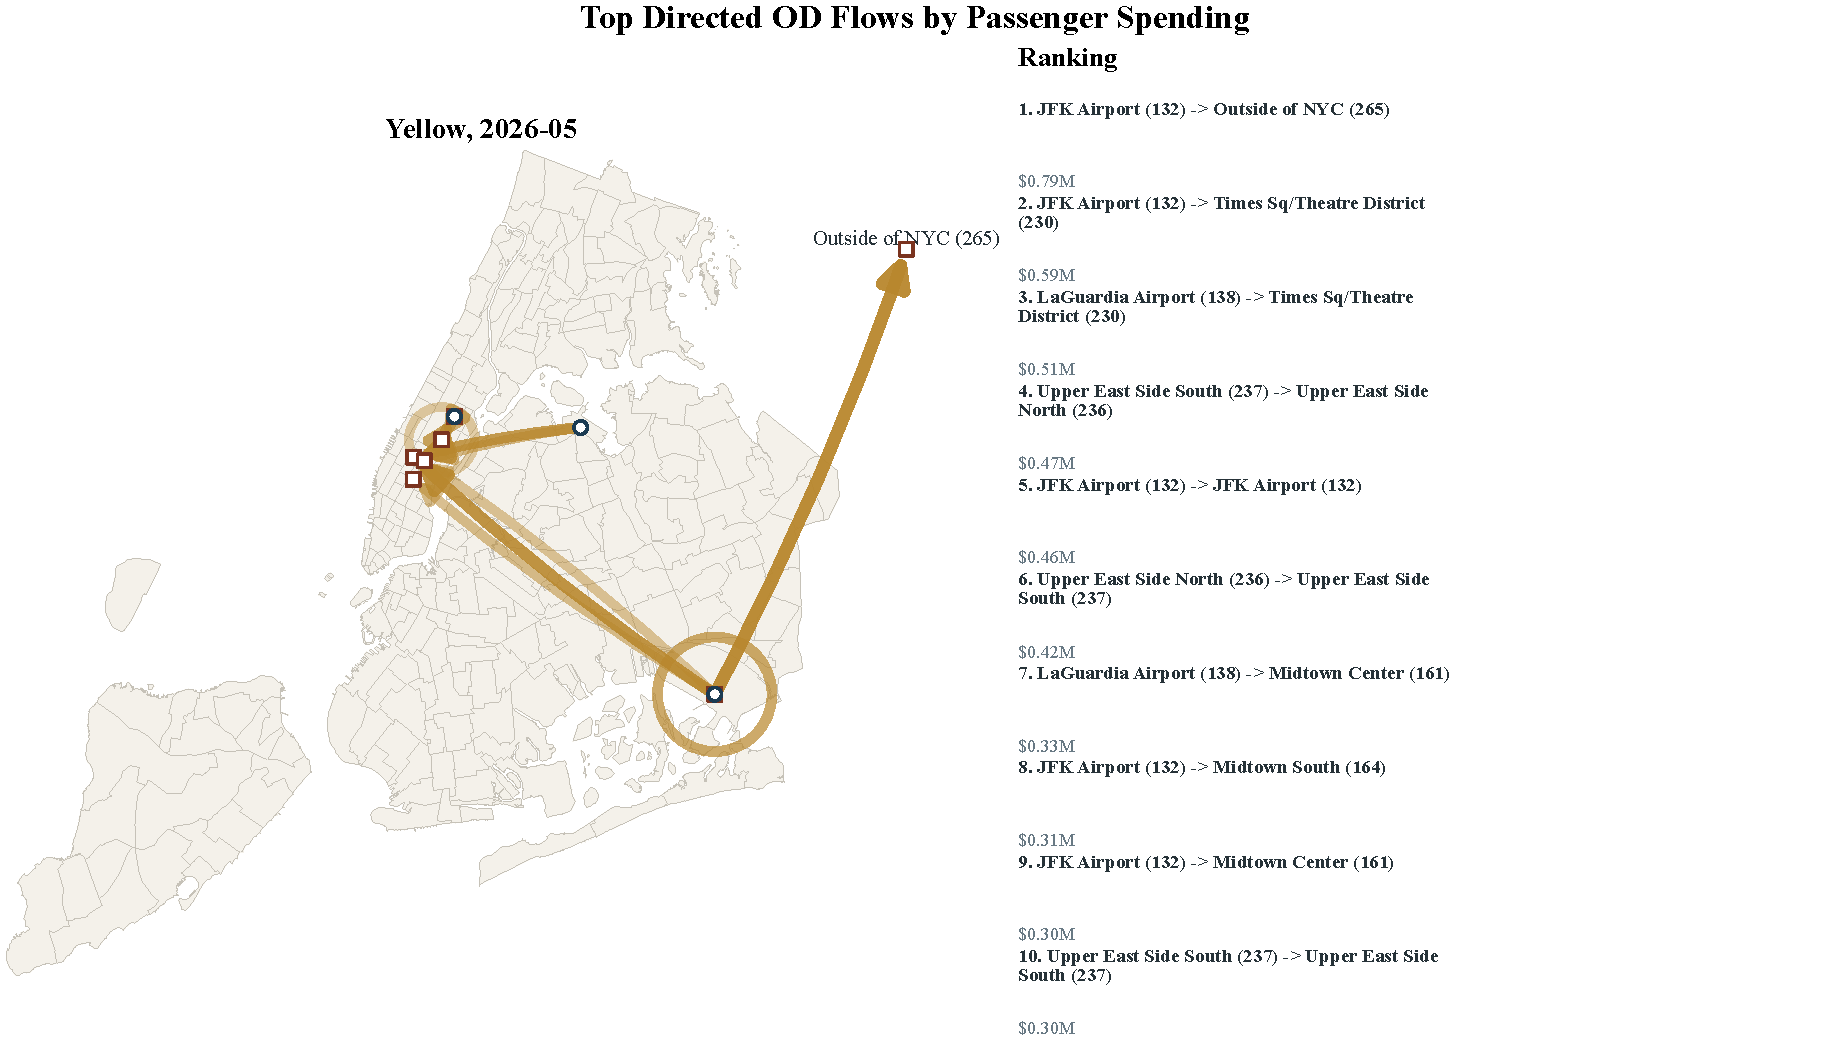
\includegraphics[height=.265\textheight,width=.98\linewidth,keepaspectratio]{04_Results/report_figures/appendix/task2_od_spending_2026-05_yellow.pdf}\par\vspace{0.2em}
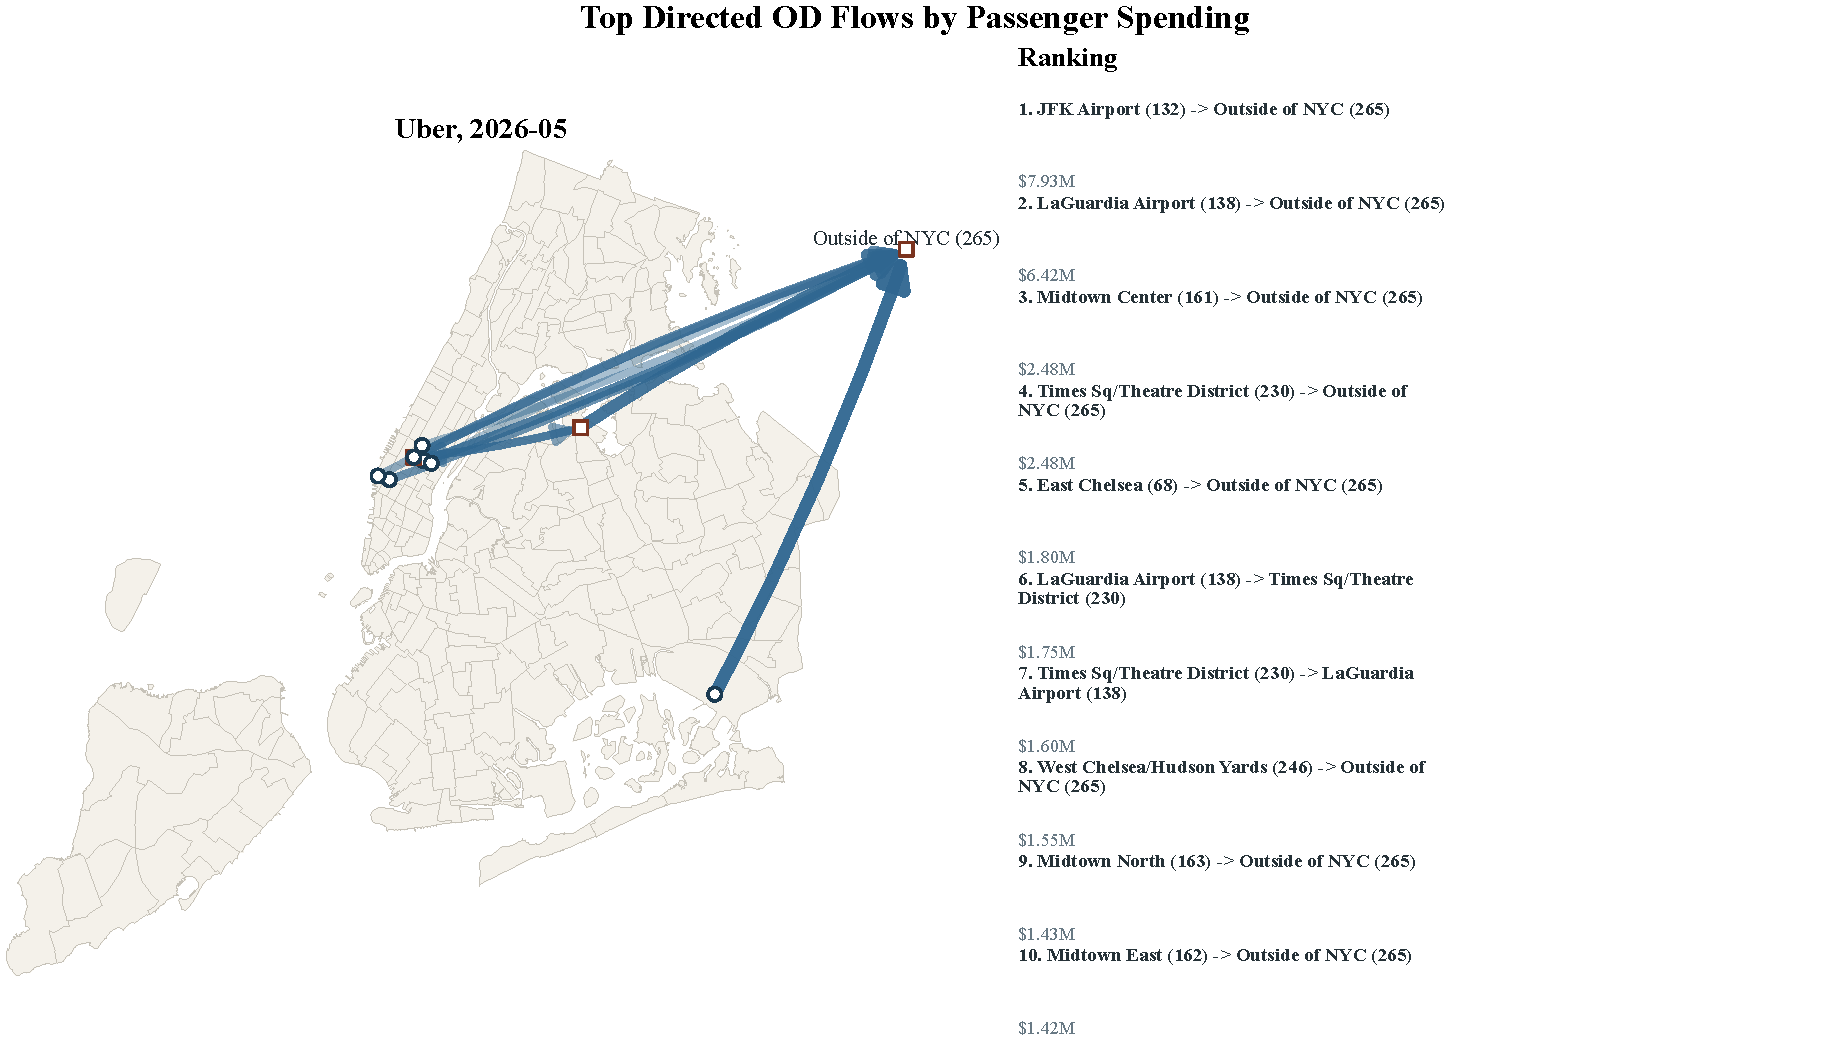
\includegraphics[height=.265\textheight,width=.98\linewidth,keepaspectratio]{04_Results/report_figures/appendix/task2_od_spending_2026-05_uber.pdf}\par\vspace{0.2em}
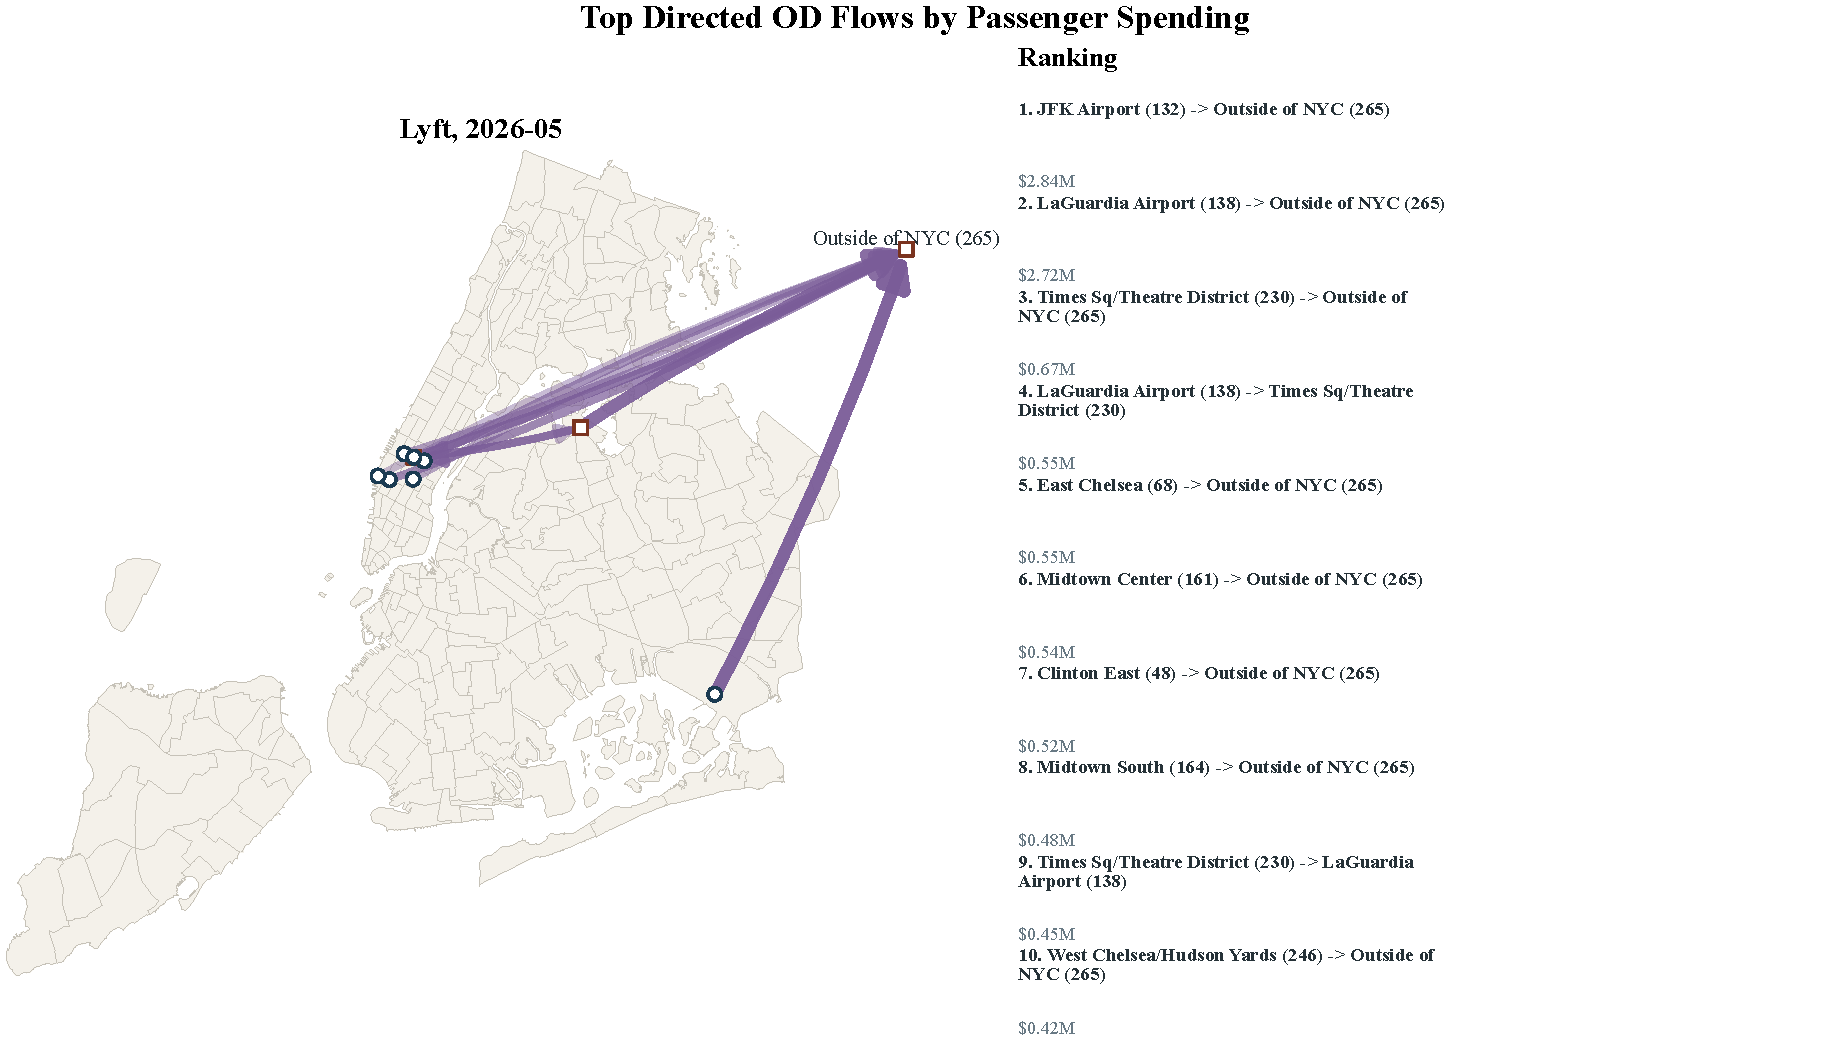
\includegraphics[height=.265\textheight,width=.98\linewidth,keepaspectratio]{04_Results/report_figures/appendix/task2_od_spending_2026-05_lyft.pdf}
\captionof{figure}{Top ten OD flows by aggregate passenger spending, 2026-05. Panels from top to bottom: Yellow Taxi, Uber, and Lyft.}
\end{center}
\clearpage

\subsection{Zone-level reported ride-pooling metrics}
Each panel reports pickup-zone request, match, and success metrics. Gray zones do not meet the required denominator threshold.

\begin{center}
\centering
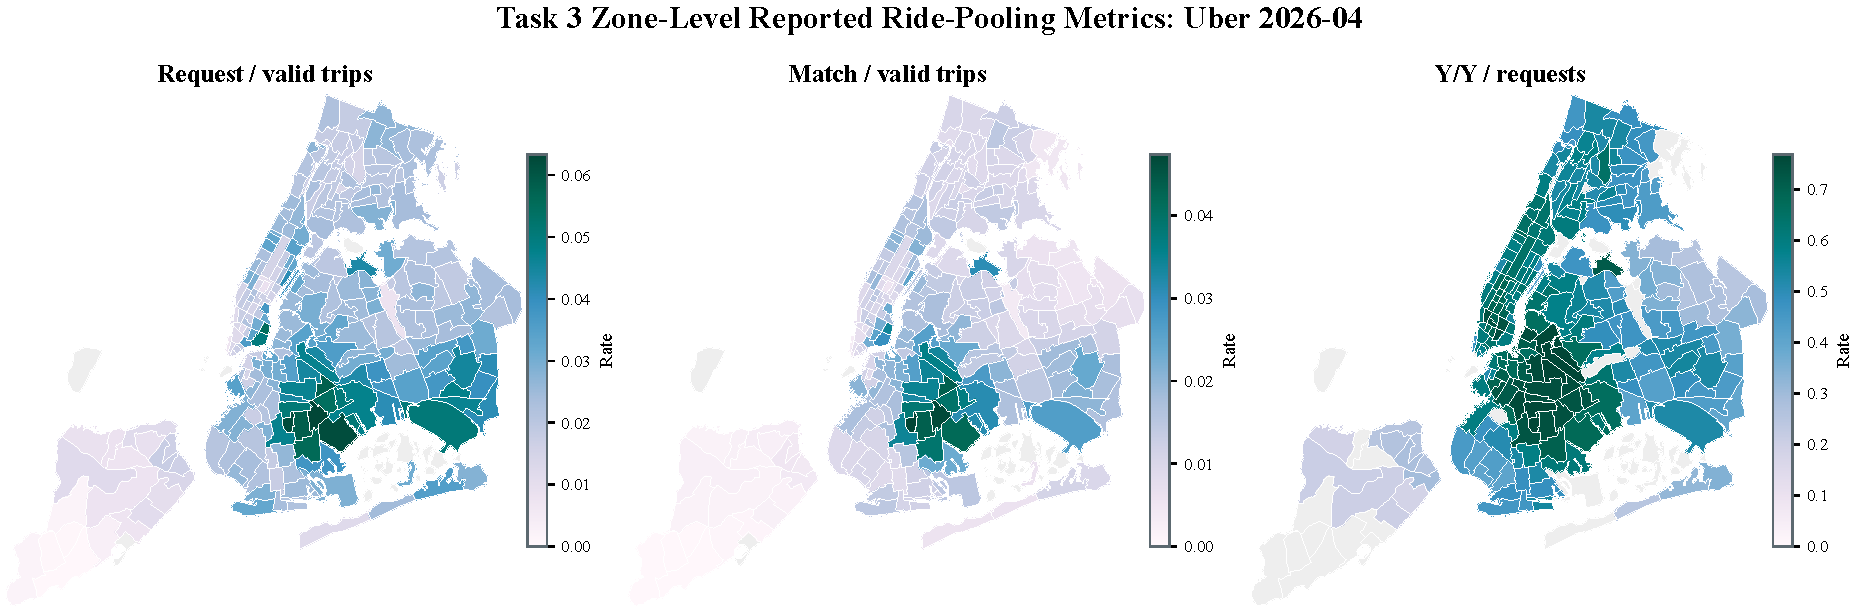
\includegraphics[height=.375\textheight,width=.98\linewidth,keepaspectratio]{04_Results/report_figures/appendix/task3_zone_metrics_2026-04_uber.pdf}\par\vspace{0.3em}
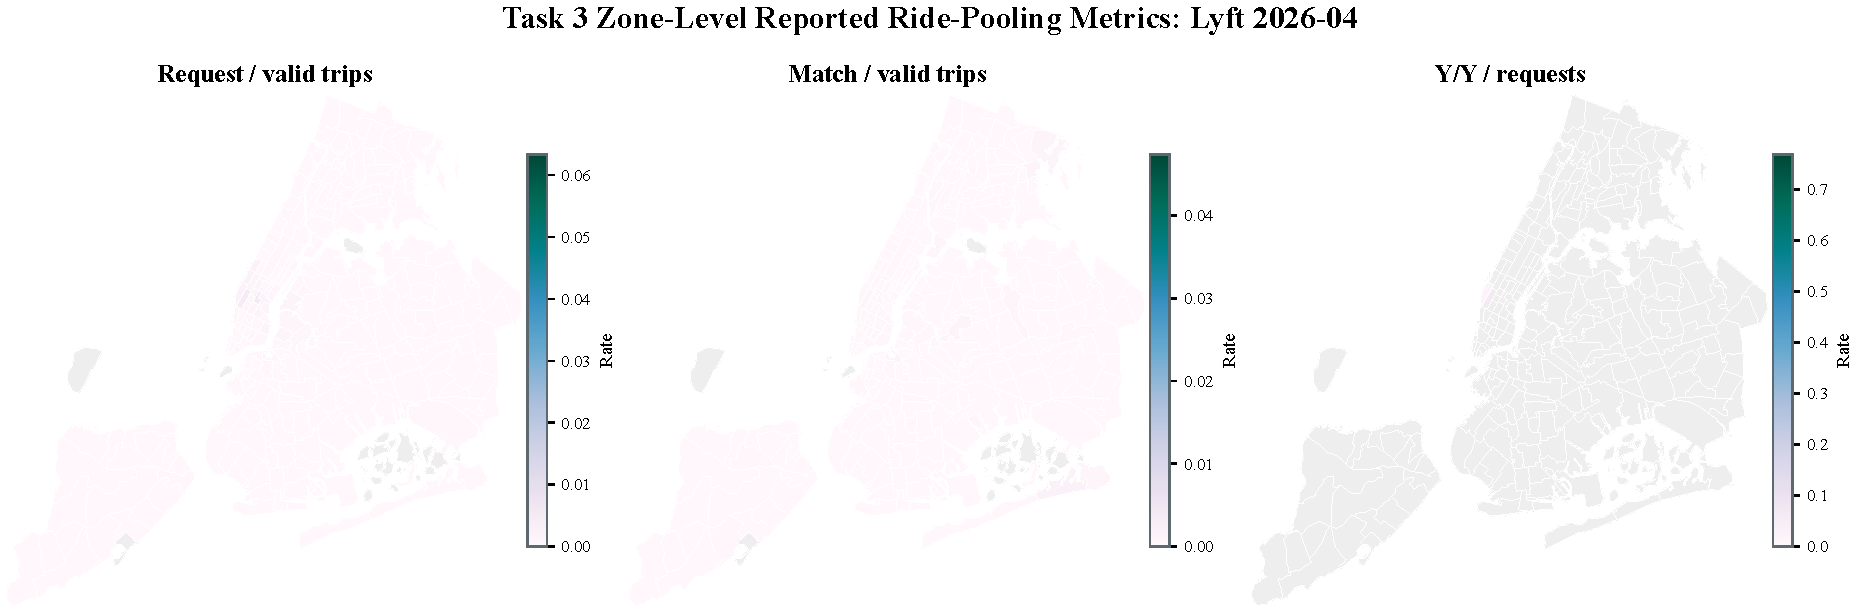
\includegraphics[height=.375\textheight,width=.98\linewidth,keepaspectratio]{04_Results/report_figures/appendix/task3_zone_metrics_2026-04_lyft.pdf}
\captionof{figure}{Zone-level reported ride-pooling metrics in 2026-04. Panels from top to bottom: Uber and Lyft. Gray zones have insufficient sample.}
\end{center}
\clearpage

\begin{center}
\centering
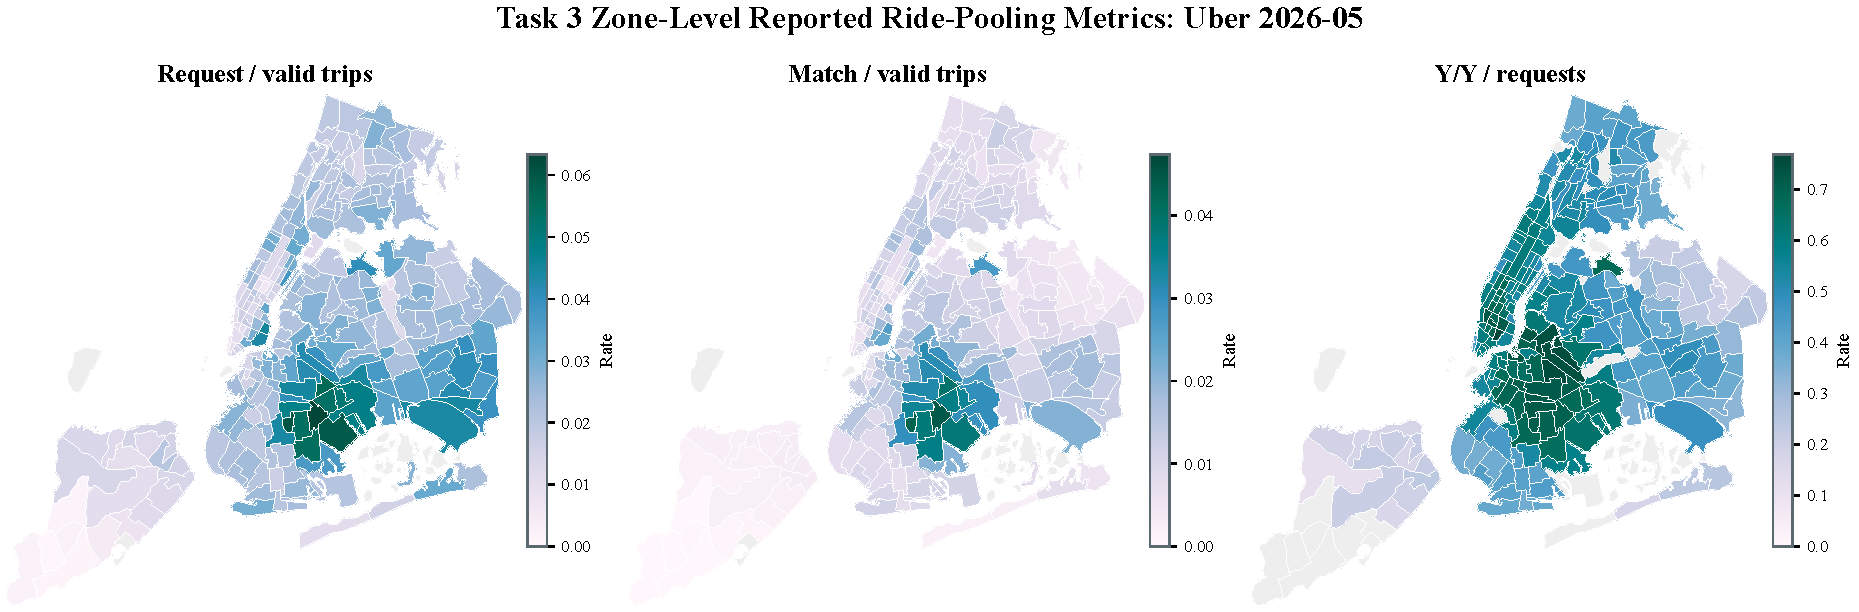
\includegraphics[height=.375\textheight,width=.98\linewidth,keepaspectratio]{04_Results/report_figures/appendix/task3_zone_metrics_2026-05_uber.pdf}\par\vspace{0.3em}
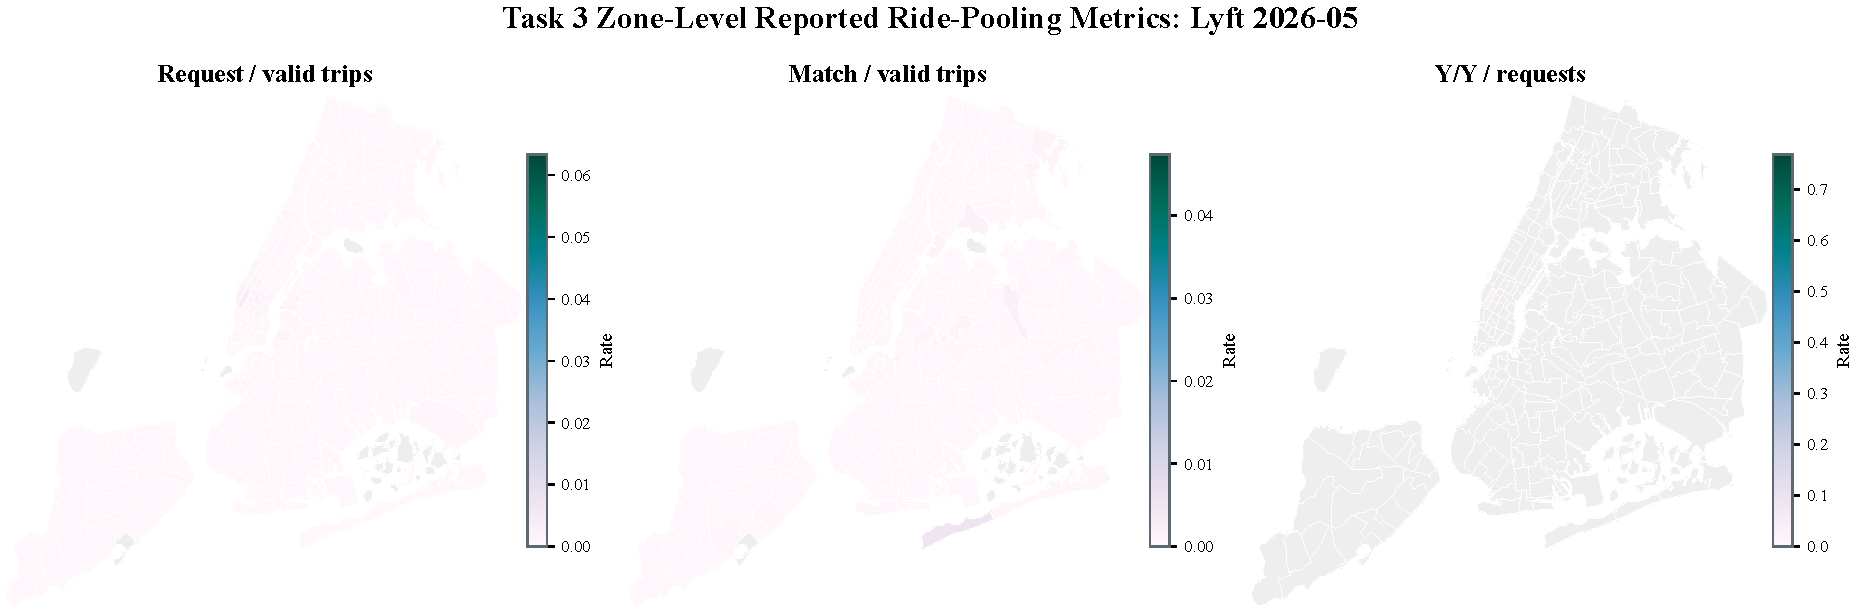
\includegraphics[height=.375\textheight,width=.98\linewidth,keepaspectratio]{04_Results/report_figures/appendix/task3_zone_metrics_2026-05_lyft.pdf}
\captionof{figure}{Zone-level reported ride-pooling metrics in 2026-05. Panels from top to bottom: Uber and Lyft. Gray zones have insufficient sample.}
\end{center}
\clearpage

\subsection{Spatial travel-time differences and reference coverage}
These maps show where supported Uber comparisons are available and how the observed mean travel-time difference varies by pickup zone.

\begin{center}
\centering
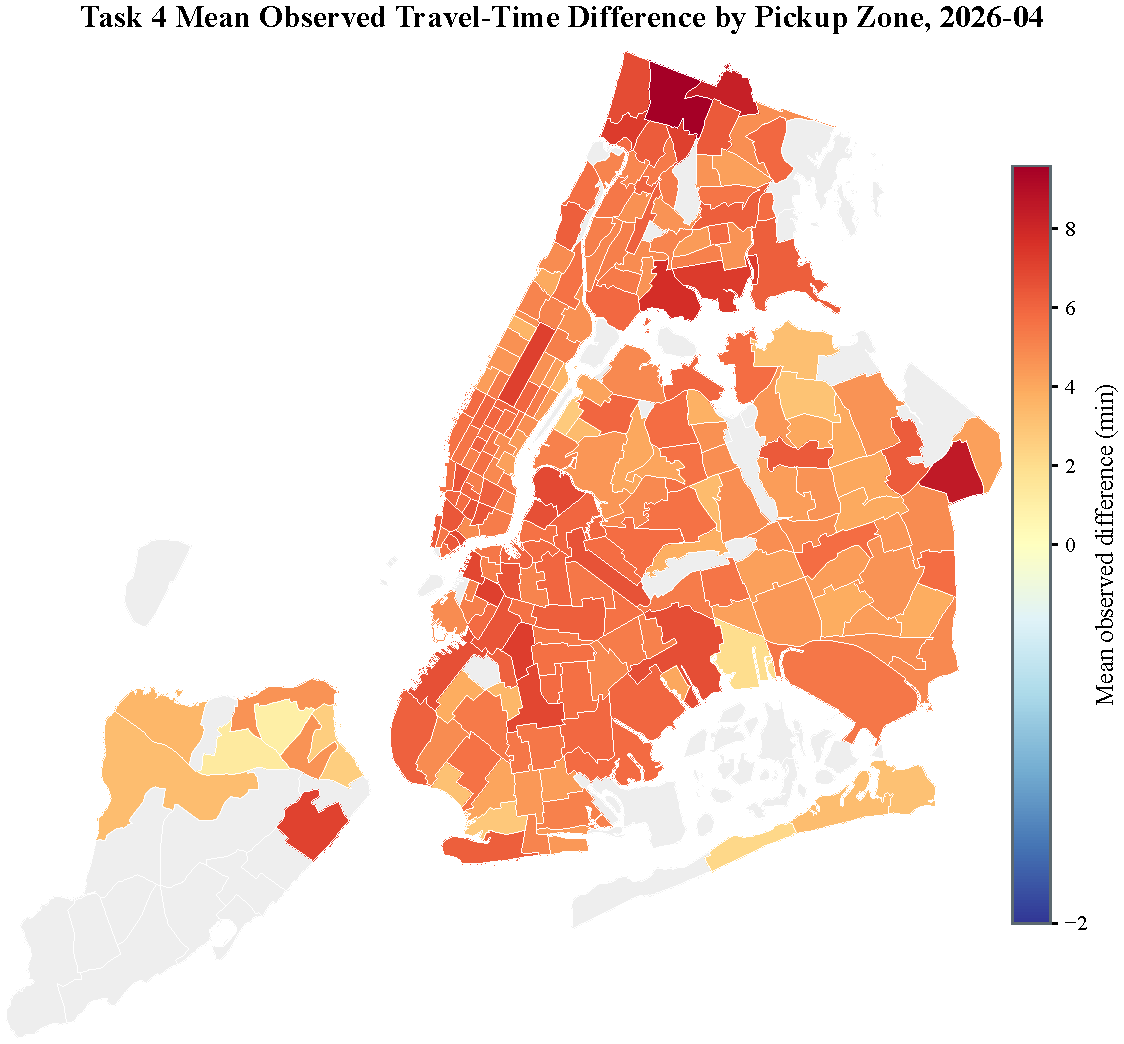
\includegraphics[height=.265\textheight,width=.98\linewidth,keepaspectratio]{04_Results/report_figures/appendix/task4_zone_mean_difference_2026-04.pdf}\par\vspace{0.2em}
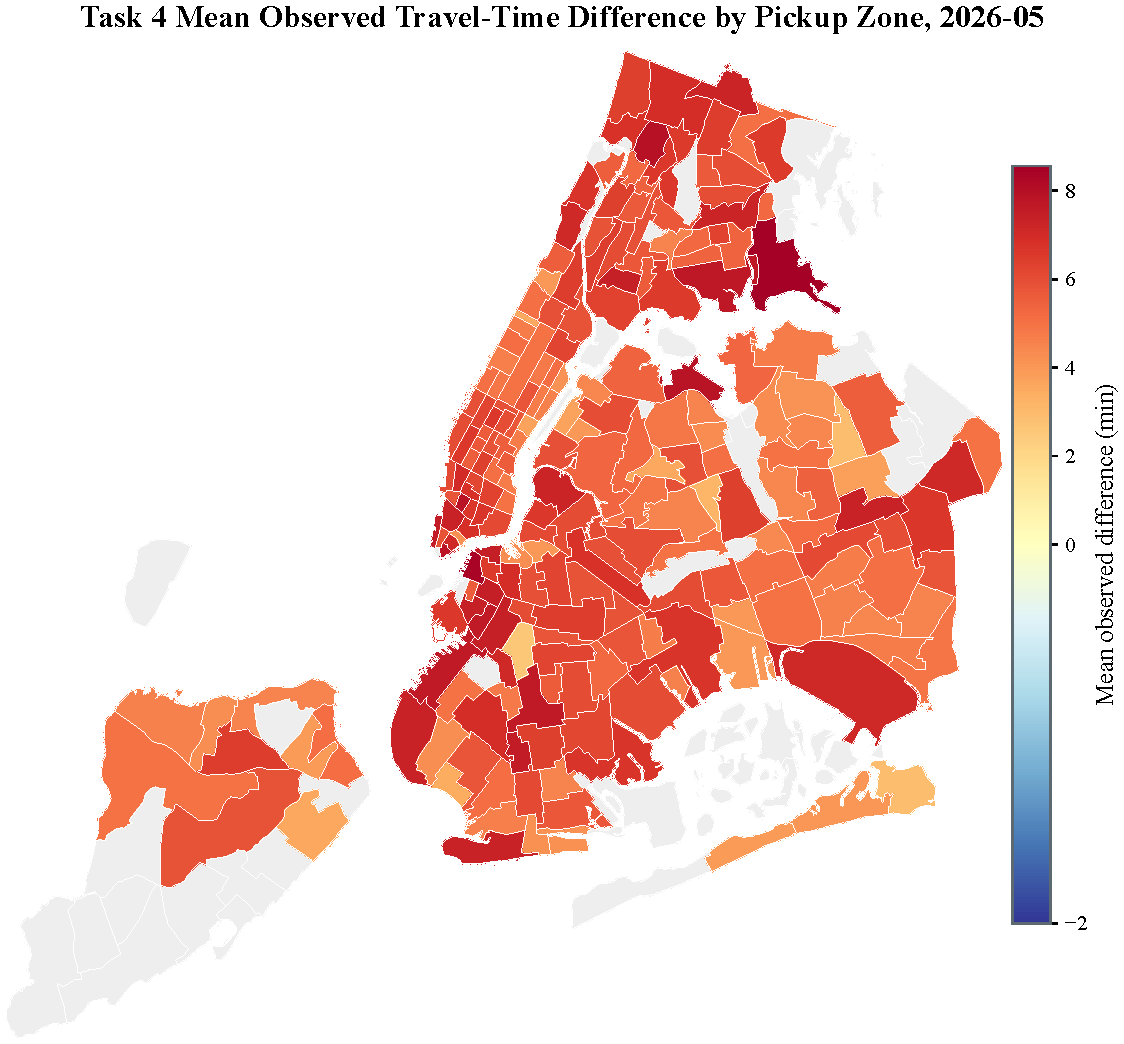
\includegraphics[height=.265\textheight,width=.98\linewidth,keepaspectratio]{04_Results/report_figures/appendix/task4_zone_mean_difference_2026-05.pdf}\par\vspace{0.2em}
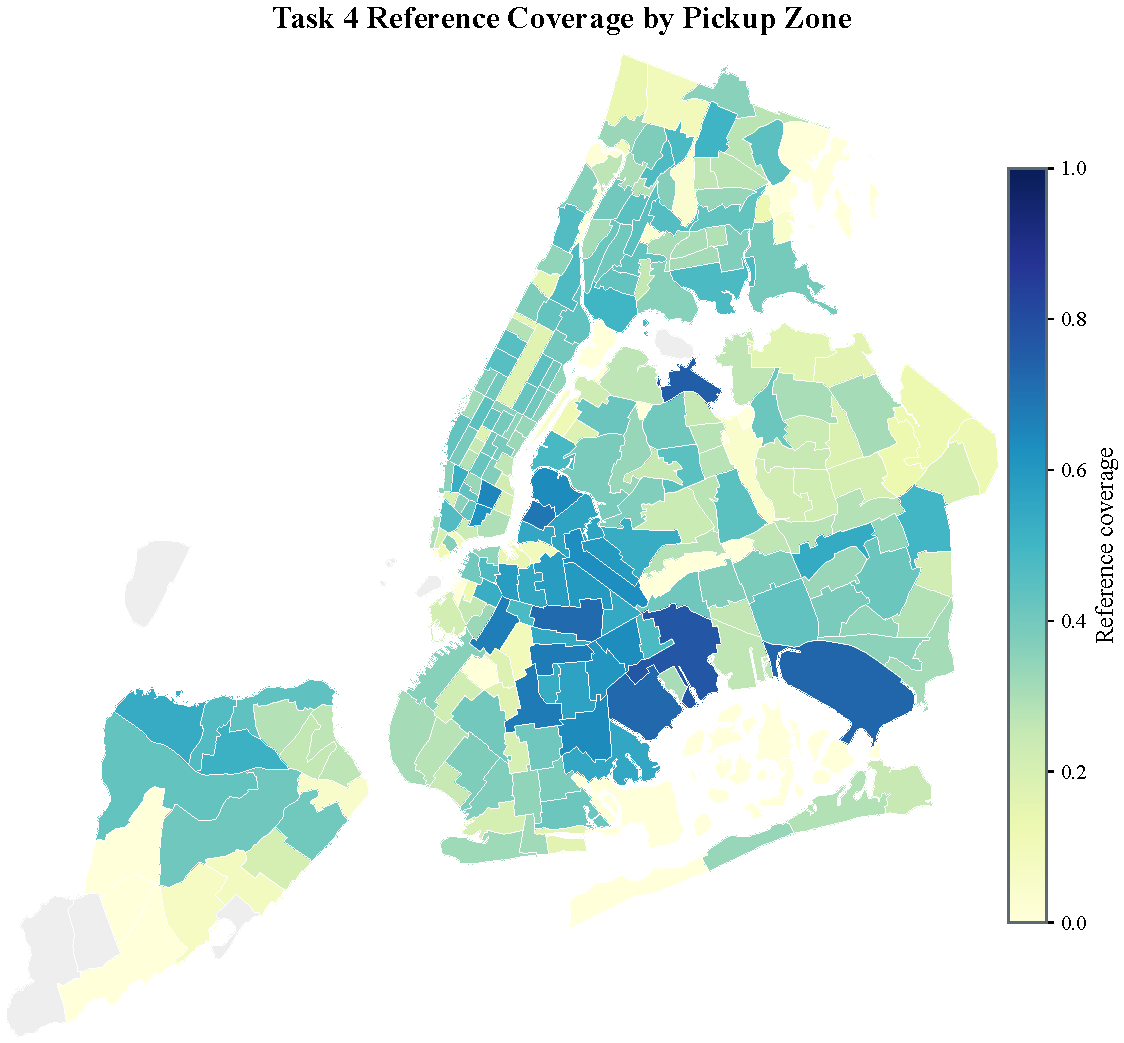
\includegraphics[height=.265\textheight,width=.98\linewidth,keepaspectratio]{04_Results/report_figures/appendix/task4_zone_reference_coverage.pdf}
\captionof{figure}{Spatial travel-time comparison diagnostics for Uber shared trips. Panels from top to bottom: April mean difference, May mean difference, and reference coverage.}
\end{center}

\endgroup


\end{document}
